
%  ********************************************************************** 


\section{Introduction}
%  ********************************************************************** 


xx
%  ====================================================================== 


\subsection{A Historical Timeline of Developmental Biology }
%  ====================================================================== 


xx
%  ---------------------------------------------------------------------- 


\subsubsection{The Science of How Organisms Form}
%  ---------------------------------------------------------------------- 


A general definition would state that \textit{development} is a dynamical process leading a given organism to a given morphological state, and that the study of development is the study of the mechanisms ruling the coordination of cellular differentiation through space and time in a multicellular organism. This process is not steady, however, and organisms may alternate periods of intense transformation with "quieter" periods dedicated to growth only. However, the most dramatic events occur in the beginning, when the egg divides into myriad of cells. These soon start to perform a collective ballet of complex movements, which are precisely coordinated through a system of physicochemical interactions. It is interesting to note that this process never ends, the morphological state of an organism undergoing constant change, albeit smaller, until senescence and death.

The definition of development has its own "embryogenesis": it has also changed through the numerous discoveries that punctuated the history of the field, and the practical methods used. Three major periods can be distinguished [ref Hopwood XXXXX]:
\begin{itemize}
	\item pre 1880: classical descriptive biology (Section 1.1.2)
	\item 1880-1930: classical experimental biology (Section 1.1.3)
	\item 1960: (modern) developmental biology (Sections 1.1.4-6)
\end{itemize}
%  ---------------------------------------------------------------------- 


\subsubsection{First Theories: Epigenesis, Preformation and Spontaneous Generation}
%  ---------------------------------------------------------------------- 


\paragraph{Aristotle Envisioned Them All}
%  ++++++++++++++++++++++++++++++++++++++++++++++++++++++++++++++++++++++ 


If Hippocrates is often labeled as the first embryologist, based on his \textit{Hippocratic Collection} where he describes the successive stages of incubation of hens' eggs \cite{Needham:1931tz}, it is Aristotle in \textit{De Generatione Animalium} who initiated the main theory of the formation of living organisms that still hold today. This theory, called "epigenesis", states that organisms develop through changes of shape. New parts appear and deform by themselves through a series of stages. In his Book II, Aristotle foresees the alternative theory of "preformation", which persisted well through the 18th century before it was gradually dismissed. It states that organisms develop from miniature versions of themselves, thus no new structures are generated during development, but parts simply unfold and grow:

   Either all the parts, as heart, lung, liver, eye, and all the rest, come into being together or in succession, as is said in the verse ascribed to Orpheus, for there he says that an animal comes into being in the same way as the knitting of a net \cite{Aristotle:WxoMhbAm}. 

A third hypothesis was developed by Aristotle in \textit{Historia Animalium}\cite{Aristotle:WxoMhbAm}. Synthesizing contemporary thought, he introduces the theory of "spontaneous generation". This theory proposes that some complex organisms, like insects, are generated from non-living matter, like putrefying earth, vegetable matter, or dead flesh.

\paragraph{Early Mechanical Interpretations}
%  ++++++++++++++++++++++++++++++++++++++++++++++++++++++++++++++++++++++ 


In 1651, William Harvey was among the first philosophers to consider embryonic development as a dynamic process requiring a causal explanation of a sequence of events \cite{Horder:2010uj}. In 1664, Ren\'e Descartes' \textit{De la formation du foetus}\cite{Descartes:1677un} was posthumously published and contained the first attempt to explain the formation of an animal embryo by means of mechanistic interactions. In this theory, the male and female seeds would heat up and ferment until some of their particles started moving and forming the organs, from the heart that pushed the blood directly towards the place it was freest to go and participate in the formation of the brain \cite{Roger:1998td}.

\paragraph{The End of Spontaneous Generation}
%  ++++++++++++++++++++++++++++++++++++++++++++++++++++++++++++++++++++++ 


In 1668, Gregorio Redi realized an experiment which discredited the spontaneous generation hypotheses by showing that no fly can form in a closed jar containing food or dead flies. As maggots would appear when the same experiment was run in an open jar, he concluded that the food or dead flies could not produce maggots by themselves \cite{Theriseofembryolo:2000uf}. The final blow to this theory was struck by Louis Pasteur two centuries later (1859) when, as a young chemist, he showed that a boiled meat broth would not produce new organisms. The game changer of his experimental setup was bending the neck of the container into a S shape. It allowed air to pass through it but not the aerial microorganisms because of gravity. However, when the inflexion point was put in contact with the broth, a culture would rapidly start to grow.

\paragraph{The End of Preformationism}
%  ++++++++++++++++++++++++++++++++++++++++++++++++++++++++++++++++++++++ 

\begin{figure}
\begin{center}
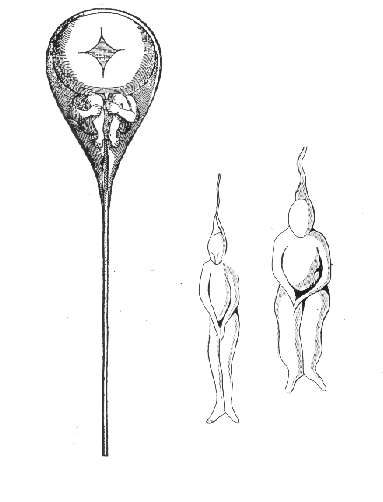
\includegraphics[width=0.5\textwidth]{../../images/Development_Review/homonculi_Hartsoecker_1695.png}
\end{center}
\caption{Drawing of the homonculi observed in sperm by Nicolaas Hartsoecker (1695)}
\label{homonculi_Hartsoecker_1695}
\end{figure}

The contention between preformists and the upholders of epigenesis lasted longer. Antonie van Leeuwenhoek was a Dutch scientist who created various microscopes. In 1676, he made the first observation of single-celled organisms, "animalcules", soon after Robert Hooke had first described and termed the "cells" \cite{Hooke:2005vy}. Leeuwenhoek discovered that the sperm cells of animals, among which humans, were entering the egg cell \cite{Gest:2004fj}. In addition to his contribution to the refutation of spontaneous generation, this discovery favored the spermist side of the preformation camp. Some of them started to describe miniatured humanoid shapes as did Nicolaas Hartsoeker in 1695 \ref{homonculi_Hartsoecker_1695}.

\paragraph{Germ Layers}
%  ++++++++++++++++++++++++++++++++++++++++++++++++++++++++++++++++++++++ 


In the 1820's, Christian Pander conducted a reinvestigation of developing chicks in egg and explained that development does not start from the formation of organs but originates from the transformation of primitive sheets of tissue, the "germ layers" \cite{Hopwood:2008wy}.

\paragraph{Cell Theory}
%  ++++++++++++++++++++++++++++++++++++++++++++++++++++++++++++++++++++++ 


  Between the 1820's and the 1850's, the cells were added as the second pillar of embryological analysis mostly under the influence of Johannes Müller \cite{Hopwood:2008wy}. In the late 1830s, the cell theory attempted to unify the development of the various observed eggs in vertebrate, and particularly in mammals. The cells become progressively the fundamental building block of the living, in every living species. Robert Remak proposed that every cells were produced by preexisting cells, starting from the egg, through the germ layers, and finally to the tissues \cite{Lagunoff:2002gw}. This insight is now called the segmentation or cleavage stage and it is indeed the first morphological event of today's developmental study. Remak also introduces the concept of germ-layer specificity in vertebrates, stating that each layer - endoderm, mesoderm, and ectoderm - is specifying the cell type (or fate) of all cells originating from it (muscles, skin, nervous system, intestine...) \cite{Remak:1855tc}. This concept is central to embryology as it preludes the fundamental questions that will occupy embryologists until then.   mendel law  -> look for cleavage  -> lignage,  -> body plan / rupture de symmetrie  -> bod  
\begin{figure}
\begin{center}
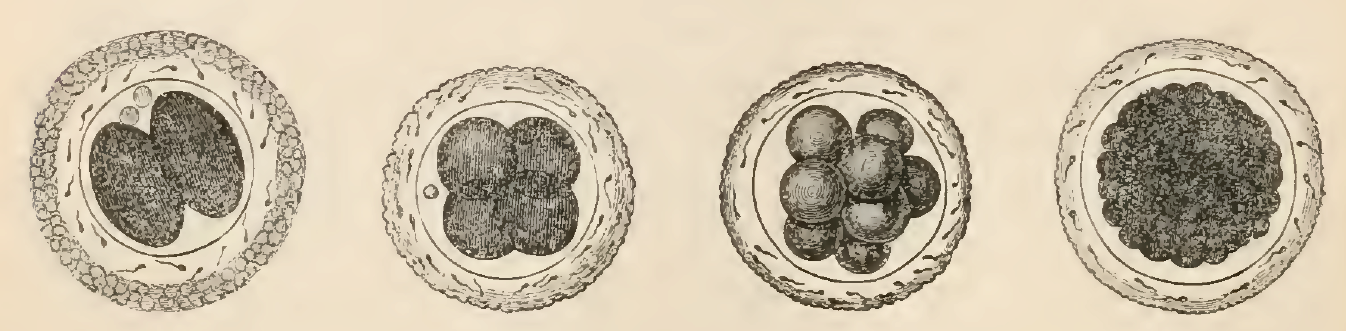
\includegraphics[width=0.7\textwidth]{../../images/Development_Review/dog_segmentation_kolliker_1861.png}
\end{center}
\caption{Egg segmentation from a dog's oviduct, surrounded by the zona pellucida and spermatozoa as represented by Albert Kölliker in 1861 \cite{Kolliker:1861uj}.}
\label{Development_Review_dog_segmentation_kolliker_1861}
\end{figure}
%  ---------------------------------------------------------------------- 


\subsubsection{The Rise of Experimental Embryology}
%  ---------------------------------------------------------------------- 


Starting in the 1880's, some embryologists reinvented their methods through experimentation to decipher the causal links between the successive stages of development. Calling this discipline \textit{Entwicklungsmechanik} ("developmental mechanics"), Wilhem Roux and others applied to embryos various kinds of perturbations, whether mechanical, thermal, chemical or electrical \cite{Hopwood:2011gt}.

\paragraph{\textit{Entwicklungsmechanik}: Self-Differentiation vs. Dependent Differentiation}
%  ++++++++++++++++++++++++++++++++++++++++++++++++++++++++++++++++++++++ 


The key question raised by Roux was whether the differentiation process of the parts of an embryo was autonomous from external influence ("autonomous differentiation" or "self-differentiation") or not ("dependent differentiation"). In 1888, he obtained half-embryos after destroying one of the cells of a two-cell frog embryo with a hot needle. The half-embryos were displaying either the anterior or the lateral halves. Roux concluded that each blastoderm was capable of \textit{self-differentiation}, independently from the missing half \cite{Hamburger:1997cm}. A year earlier, in 1887, Laurent Chabry had been the first to characterize the autonomous differentiation of cells' fate. By killing two identified blastomeres at the 8-cell stage of the ascidian tunicate, the animal became a tadpole that was missing its tail muscles. When he extracted and cultured the same two blastomeres at the same stage, they resulted in an isolated tail muscle \cite{Lawrence:2006ke}.

In 1891, following Roux's influence, Hans Driesch repeated the experiment on a two-cell stage sea urchin embryo. He separated both blastomeres and observed that each one had differentiated into a half-sized, yet complete, sea urchin larva. In 1893, by pressing on a sea urchin embryo at the third cell cycle, Driesch completely modified the relative positions of the cells and still obtained normal larvae. A mosaic determination process would have produced a highly perturbed embryo, therefore it proved that the determination occured later than expected via \textit{dependent differentiation}. Driesch concluded: "The relative position of a blastomere within the whole will probably in a general way determine what shall come from it."

These historical experiments epitomized the concurrent interpretations of autonomous vs. dependent differentiation, where the former requires "determinants" to be present at the earliest stage and separated by cell division to spatially specify cell fates, whereas the latter depends on the interaction between the cells (see a classification in \cite{Davidson:1991uu}). Later, it was recognized that truth resided in the middle. Neither totally mosaic nor totally regulative, developmental principles are a fine balance between both principles \cite{Lawrence:2006ke}. Some cells at certain stages seem highly dependent from their surroundings, and other times they seem to "seal their hatches" and follow their own differentiation path. From there on, most embryological studies will be dedicated to deciphering the modus operandi of these mixed principles, from their macroscopic characterization at the tissue level down to the molecular mechanisms at the sub-cellular level.

\paragraph{Morphogenetic Fields}
%  ++++++++++++++++++++++++++++++++++++++++++++++++++++++++++++++++++++++ 
  XXXXX René arrete ici : toute la suite à rédiger...  Autonomous vs Conditional specification/specialisation/determination/differentiation (yields concept of induction, determination, competence, potentialities, regulation, diffusion, morphogenetic fields, gradients...): maybe the most fundamental concept of development, developmental concept in its own right (not borrowed to another discipline). at the tissue level and at the cellular level.  Here we must define the notion of competent tissue and induction XXXX -> gradients, fields, competence, induction, differentiation, commitment, specification, determination, specialization, canalization, regionalization, potential  Fields  

  The early 20th embryologists refined these question with new experiments as grafts and aimed at deciphering what determine the cell fates. In 1918, Ross Harrison publish a paper which introduced the concepts of morphogenetic fields \cite{Harrison:1918ta}. He experimented various limb grafts on newt embryo. He grafted some cells from a specific region of the mesoderm to the non-neural ectoderm and observed that an additional forelimb was formed. The original grafted cell population has the ability, even after transplantation, to "remember" its fate. Even if the cells were separated in two subpopulation and grafted independently, both grafts would grow intact limb \cite{DeRobertis:1991ua}. The key property of a morphogenetic field is to conserve its potential even after important manipulation. Later observations shown that the fate of the morphogenetic field was depending on the position along the antero-posterior axis. It lead to the notion of gradient-field which determines the identity of the fields \cite{huxley1934elements}. 

\paragraph{Induction}
%  ++++++++++++++++++++++++++++++++++++++++++++++++++++++++++++++++++++++ 


  In 1924, Hans Spemann and his PhD student Hilde Mangold reported the discovery a tissue in the Newt gastrula which, when grafted on the ectodermal region of another Newt embryo, triggers a neurulating process and initiates the formation of a secondary embryonic axis \cite{Spemann:1924ky}). This tissue was denominated the \textit{organizer} as it was able to instruct and organize the adjacent ectoderm. Spemann proposed two different speculative mechanisms: either the existence of a chemical substance that would be transmitted to the induced tissue or the inducing tissue would possess a specific vitalistic "structure" associated to the living embryo \cite{Holtfreter:1991wi}. These hypotheses became the focus of intensive study around the world. 

  Boiling, dessicating and other tissue killing experiment exercised on the Spemann organizer rapidly dismissed the second hypotheses. A variation of the theme of induction was introduced by Waddington's "Organisers and Genes" \cite{Waddington:1940tj}, the "evocator-comptence system" would state that the inducing substance, i.e. the evocator, was only slightly perturbing the dynamics of the competent tissue, which would actively respond by a change a state controlled by the genes \cite{Gilbert:1991ww}. The organizer was not any more actively organizing the formation of the induced organs but simply releasing a water-diffusible chemical agent which would initiated the self-organization of the induced tissue. A global quest on the identity(ies) of the inducing substances started around the world . Johannes Holtfreter used dead or desintegrated organizer tissue that still induced neurulation (1932) \cite{Gerhart:1998wy}, multiple chemical substances were diffused into the competent tissue \cite{Steinbeisser:1996vs}): lipids \cite{Needham:1934ux}, oleic and nucleic acids \cite{Wehmeier:1934wh}, proteins \cite{Barth:1938fx}, activin (a mesoderm inducing protein from chicken) \cite{Tiedemann:1992te}, follistatin (as it became evident that induction was occuring in multiple tissues \cite{Kessler:1994un}, ubiquitous candidate substances was targeted)... Later, in 1961, Lauri Saxon showed that the inducing substance could act through "millipore" filter with an average pore size of 0.8 micron and a thickness of 20 microns, confirming that the substance was indeed diffusive \cite{Saxen:1961uk}. 

  Decades later, the variety of candidate substances positively inducing neurulation progressively discouraged the embryologists to elucidate the quest of finding tissue-inducing agent and the more promising field of modern molecular biology attracted the younger ones away from this quest \cite{Holtfreter:1991wi}. However, the concept of induction was only suffering a temporary slowing down, before witnessing a rebirth and eventually being grounded in physico-chemical terms. 
%  ---------------------------------------------------------------------- 


\subsubsection{Developmental Genetics}
%  ---------------------------------------------------------------------- 


  In the early 20th century, embryology and genetics were both part of the larger field of heredity and were tightly entangled. A split was initiated by the work of Thomas Morgan who proposed that, to avoid confusion, embryology would study the expression of the hereditary traits whereas genetics would deal only with the transmission of those traits (see Chapter II of "The Theory of the Gene" \cite{Morgan:1926wt}). From this time, some biologists tried to reunite both fields, leading the emerging field of developmental genetics.  

  The first publication which founded this field is the work of Gluecksohn-Schoenheimer which interpreted the defect in the induction of the mouse notochord as the consequence of a mutation of the Brachy gene (1938, 1940) \cite{GluecksohnSchoenheimer:1938vk}, \cite{GluecksohnSchoenheimer:1940wg}. The result would not only pioneered developmental genetics but it also proposed a new methodology for the study of embryology. Instead of perturbing experimentally the development of embryo and observe the consequences on the phenotype, mutant phenotype were to be observed first and genetic causes had to be decipher from it. 

  This methodological dichotomy would merge decades later with the experimental generation of mutants selected by the observation of their phenotypes. (like chemically induced random mutation in \textit{Drosophila} by Nüsslein-Volhard and Wieschaus in 1980 \cite{NussleinVolhard:1980wg} or in Zebrafish a few years later \cite{NussleinVolhard:2012kb}). 

  Waddington was also an important defender of the importance of genes in development. According to him, genes act as controller of the cellular fate. By comparing the development of mutated \textit{Drosophila}, he observed that a presumptive tissue (the imaginal disc) would transform into a leg or an antenna according to the mutation \ref{{Gilbert:1991ww}}. He illustrated his views by the concept of epigenetic landscape and canalization which shows foldings on a hill side that guide the fate of cells. Under the hill, the genetic interactions reshape the foldings to organize embryonic development (Fig. \ref{Development_Review_waddington_epigenetic_nature_mod_small_intro}).  
\begin{figure}
\begin{center}
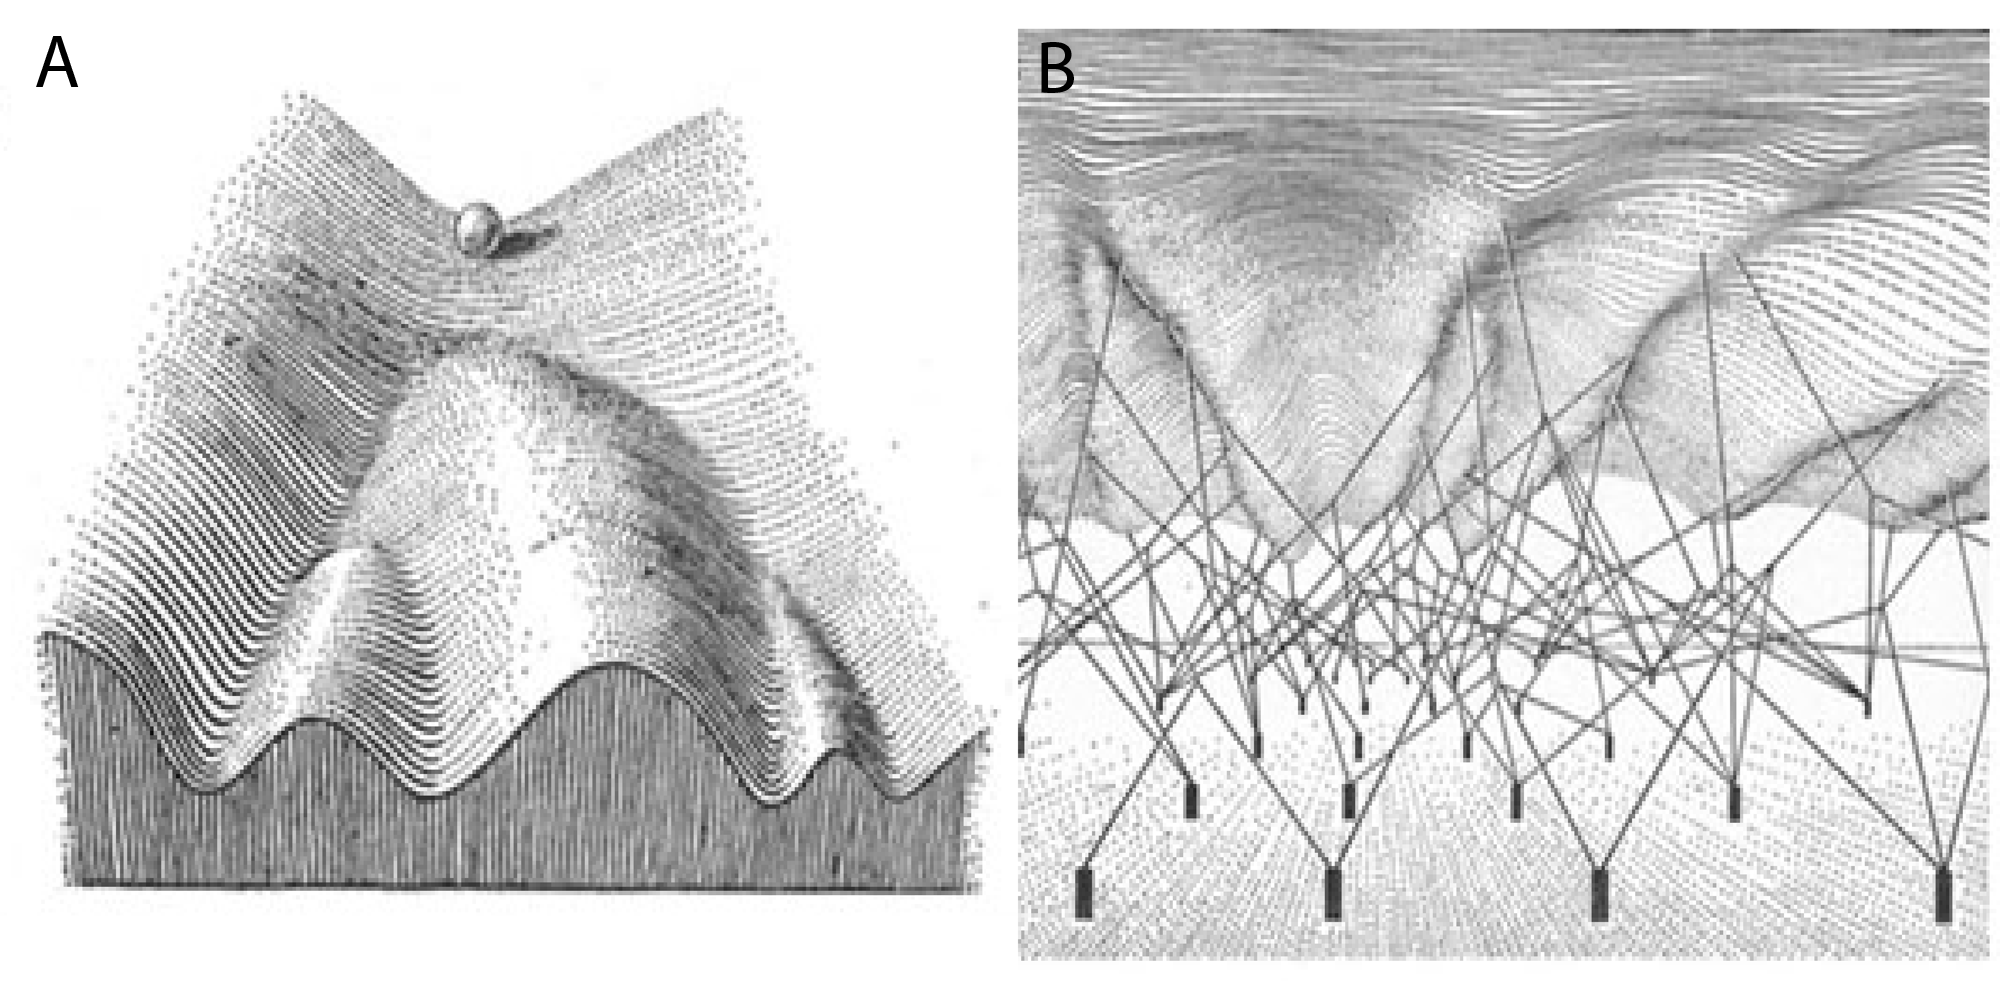
\includegraphics[width=0.8\textwidth]{../../images/Development_Review/waddington_epigenetic_nature_mod_small.png}
\end{center}
\caption{\textbf{Waddington's epigenetic landscape.} A: The ball represents a cell evolving in the epigenetic landscape. Its fate is determined by the canals in which the ball is rolling. B: A view of the landscape's behind the scene. The landscape relief is dynamically controlled by hidden wires which symbolized the gene expression and interactions. Image and legend adapted from Slack \cite{Slack:2002kg}}
\label{Development_Review_waddington_epigenetic_nature_mod_small_intro}
\end{figure}
%  ---------------------------------------------------------------------- 


\subsubsection{Molecular Genetics}
%  ---------------------------------------------------------------------- 


\paragraph{Operon-Lactose}
%  ++++++++++++++++++++++++++++++++++++++++++++++++++++++++++++++++++++++ 


  The discovery of the operon-lactose mechanism initiated the genetic trend in embryology. It applied the mechanism of induction at the sub-cellular level by introducing genetic determinants, the \textit{regulator and operator genes}, which control the rate of protein synthesis through the action of \textit{repressors}\cite{JACOB:1961uh}). This seminal paper already envisioned the influence of this discovery on embryology: 
\begin{quotation}  The occurrence of inductive and repressive effects in tissues of higher organisms has been observed in many instances (...). It has repeatedly been pointed out that enzymatic adaptation, as studied in micro-organisms, offers a valuable model for the interpretation of biochemical co-ordination within tissues and between organs in higher organisms. The demonstration that adaptive effects in micro-organisms are primarily negative (repressive), that they are controlled by functionally specialized genes and operate at the genetic level, would seem greatly to widen the possibilities of interpretation. The fundamental problem of chemical physiology and embryology is to understand why tissue cells do not all express, all the time, all the potentialities inherent in their genome. 
\end{quotation}

  Immediately understood by some embryologists as Waddington who had defended the notion of a cytoplasmic activated, genetic control of the cell fate in development (Chapter "The Activation of Genes by the Cytoplasm" in "Principles of Embryology", 1956 \cite{Waddington:1956wf}, this discovery opened the door to the reconciliation between the embryology orchestration of spatio-temporal cell specification and the biophysical molecular paradigm. 

\paragraph{Gene Regulatory Networks (GRNs), \textit{Cis}-Regulatory Systems}
%  ++++++++++++++++++++++++++++++++++++++++++++++++++++++++++++++++++++++ 


  The modern view of the orchestration of the cell behavior in space and time is conceptualized by the work of Eric Davidson on the cis-regulatory system. It is an extension of the work of Jacob and Monod which systematizes the role of the genes' regulators, as arrays of transcription factor target sites on the DNA molecule \cite{Arnone:1997th}. These arrays, called the \textit{cis-regulatory elements} as they are usually on the same DNA molecule as the genes they regulate \cite{Davidson:2006ud}, define a network of interaction between the genes involved in development. This network is called the \textit{gene regulatory network} (GRN) and its dynamics is regulated by the topology of the GRN and the quantities of the various \textit{transcription factors} (TFs) that bind the cis-regulatory elements. As E. Davidson mentioned, the first GRN were anecdotal, but since 2002, rapid improvement in their systematic analysis lead to the publication of large scale networks, such as the network specifying the endomesoderm of the sea urchin embryo (more than 40 genes), or the network responsible for the dorsoanterior-ventroposterior patterning and the endoderm formation of the zebrafish embryo \cite{Chan:2009er}. 

\paragraph{Maternal Factors}
%  ++++++++++++++++++++++++++++++++++++++++++++++++++++++++++++++++++++++ 


  The dynamics of the GRN regulation is initialized by the various \textit{maternal factors}\cite{Pelegri:2003wm}. The transcription factors are already present in the egg and serve as inputs of the GRN. The first direct evidence of a maternal RNA present in the oocyte and control the early activation of the GRN in the mouse was published in 1994 \cite{Renard:1994wo}. Maternal factors anisotropy is also an important concept yielding the patterning of the body plan. As the maternal factors are not homogeneously spatialized in the egg, a differential initialization of the GRN occurs in the different blastomeres. The \textit{bicoid} gradient establishes the antero-posterior axis in the \textit{Drosophila} embryo and is responsible for many asymmetries \cite{Gavis:1992ug}\cite{StJohnston:1992uu}. In the \textit{Caenorhabditis elegans} nematode development, the \textit{Skn1} maternal factor is concentrated at the posterior axis and specify the antero-posterior axis \cite{Bowerman:1992tc}. In the zebrafish, a maternal transcript, \textit{Squint}, has been proposed as a predictor of the dorsal axis \cite{Gore:2005fj}. 

\paragraph{Gene Regulatory Networks and Epigenetics}
%  ++++++++++++++++++++++++++++++++++++++++++++++++++++++++++++++++++++++ 


  Recent discoveries emphasize the role of epigenetic phenomena during the embryonic development. These mechanisms introduces novel possibilities to control the genetic expression during development. Among these mechanisms, we mention DNA and histone methylation in zebrafish \cite{Lindeman:2010ia}\cite{Lindeman:2011fn}), control of the transcriptional activity by perturbating the nuclear envelope with mechanical forces exerted by microtubule polymerization in \textit{Drosophila}\cite{Hampoelz:2011wv}, and genes silencing by RNA interference in \textit{Drosophila}\cite{Yamanaka:2012da}. 

\paragraph{Signaling Pathways, Transduction}
%  ++++++++++++++++++++++++++++++++++++++++++++++++++++++++++++++++++++++ 


  The GRN dynamics view is centered on the cell, but it also integrate their communication capabilities through exchange of molecular information. These cell-cell interactions are realized by the binding of a secreted extracellular ligand which triggers a transduction and a modification of the cytoplasmic dynamics. As mentioned Pires-daSilva and Sommer, a wide variety of cells uses only a few classes of \textit{signaling pathways}\cite{PiresdaSilva:2003bj}. Among these pathways, the \textit{Wnt} gene has been discovered multiple times in different animals. Its name itself is the contraction of the two occurrences \textit{Int1} which was characterized in 1982 by Nusse and Varmus as a gene inducing mammary gland tumours in mice \cite{Nusse:1982wu}) and its homologue \textit{Wingless} (\textit{Wg}), described in 1973 as a gene provoking \textit{Drosophila} wings'lacking mutants \cite{Sharma:1973wy}. The \textit{Wg} mutation was later associated with default in the \textit{Drosophila} segmentation process \cite{NussleinVolhard:1980wg}). The other major signaling pathways are \textit{Notch}\cite{ArtavanisTsakonas:1999ts}\cite{Bray:2006fe}\cite{Fuss:2002vw}, \textit{Hedgehog}\cite{Wicking:1999ju}\cite{Jiang:2008ia} and \textit{TGFβ-BMP}\cite{Wu:2009ih}. 

\paragraph{Mechanotransduction}
%  ++++++++++++++++++++++++++++++++++++++++++++++++++++++++++++++++++++++ 


  Another factor of the cell dynamics is the integration of mechanical forces by the cell, \textit{mechanotransduction}\cite{Orr:2006cr}\cite{Jaalouk:2009jn}\cite{Wozniak:2009cu}\cite{Eyckmans:2011fy}. Mechanical forces have been thought as actors of tissue and organs shaping since the end of the 19$^\textrm{th}$ century, from Wolff studying the impact of the mechanical environment on the structure of bone tissue after healing of fractures \cite{wolff1892gesetz} to Roux \cite{Roux:1895vb} and D'Arcy Thompson \cite{thompson1992growth}. More recently, forces have been demonstrated to influence of vascular endothelial function \cite{Franke:1984gc}. Tension applied has been correlated with the proliferation rate in endothelial cells \cite{Nelson:2005dd} and with branching process morphology \cite{Gjorevski:2010gb}. 

  In the context of embryology, studies have demonstrated the role of forces on the cytoskeletal dynamics in the \textit{Drosophila} mesoderm invagination \cite{Martin:2010je}\cite{FernandezGonzalez:2009hp} and on the orientation of polarization axes in collective migration behaviors \cite{Weber:2011hi}. The major example of mechanotransduction has an direct input of the GRN is given by Desprat et al. \cite{Desprat:2008ei}, they showed how compression forces exerted by a tissue can induce the expression of a transcription factor in another tissue. The TF, \textit{Twist}, is involved in the differentiation of the anterior midgut in \textit{Drosophila}. After removing the pushing cells by laser ablation, they were able to rescue the Twist expression by experimental exerting forces with magnetic microtweezers. 
%  ---------------------------------------------------------------------- 


\subsubsection{Cell Biomechanics}
%  ---------------------------------------------------------------------- 


  In addition to the genetic and molecular aspects, a characteristic feature of the study of development is the study of the biomechanical properties and functions of the cells. As reviewed by Ray Keller \cite{Keller:2012ge}, this field has stayed quiet for a long time during the 20th century but has become more and more vigorous recently. Keller discriminates two tendencies which structure the physical shaping of embryos and which were both envisioned by Johannes Holtfreter: the notion of "selective affinity" modulated by adhesion and the notion of the physical integration of multiple local cellular behavior. 

\paragraph{Differential Adhesion Hypothesis and Improvements}
%  ++++++++++++++++++++++++++++++++++++++++++++++++++++++++++++++++++++++ 


  Holtfreter used his experimental skills to separate cells from their different germ layers and mix them. He observed that they were able to recognize their lineage origins and they would adopt different preferential association or "affinities" according to it \cite{Holtfreter:1939wb}. He postulated that this mechanism could lead to the progressive organization of the embryo. From 1962, Malcom Steinberg refined this idea and developed the \textit{Differential Adhesion Hypothesis} (DAH)\cite{Steinberg:1962ww}\cite{Steinberg:1963tu}\cite{Steinberg:1970bq}. Relating the behavior of cell during development to the properties of liquids, the DAH states that in heterogeneous population, cells are both cohesive and mutually motile and the interfacial surface tension will lead the ensemble towards the most stable configuration. The main factors defining the interfacial surface tension was originally the mutual adhesivity between cells, cells having a higher affinity meaning a stronger adhesive bonds. This theory had a great influence because of the simple causal link it introduced between gene expression and physical shaping rule through adhesion-molecule. Later refinements added the cell rigidity as a key factor to the interfacial surface tension definition. Through cortical tension, the principle become that stronger adhesion is increasing the contact size whereas stronger cortical tension decreases it \cite{Lecuit:2007cw}\cite{Kafer:2007do}\cite{Manning:2010ce}\cite{Maitre:2012cm}. 

\paragraph{Diversified Cell Behaviors}
%  ++++++++++++++++++++++++++++++++++++++++++++++++++++++++++++++++++++++ 


  The second notion envisioned by Holtfreter was that cell mechanical behavior was truly diversified and that the collective integration of the local behaviors was to be deciphered. He observed the specialization of the external layer of the frog gastrulae, its organization as planar sheet whom particular cell shape changing must express particular cell mechanical behaviors. The so-called \textit{epithelial} are characterized by a strong polarization between the interior side, or \textit{basal} side, and the exterior side, or \textit{apical} side. They have a strong cohesion at their lateral interface and thus form surface layers \cite{Apodaca:2012hn}. During embryonic development, epithelial behaviors may be temporary as epithelial cell may leave the surface layer and migrate toward different region. These cells are called \textit{mesenchymal} and the transformation is the \textit{epithelial-mesenchymal-transition}. Holtfreter also observed the protrusive activities of these cells in culture and the way they exert forces of the substrate and orient their migration. Trinkaus determined the migrating behavior of cells in the avian neural crest, echinoderm mesenchyme and the teleost fish epiboly \cite{Trinkaus:1984uh}. The collective behavior of mesenchymal cells have been reviewed in \cite{Weijer:2009hy}\cite{Ilina:2009dx}\cite{Rorth:2009gl}\cite{Vedula:2012ja}. 
%  ====================================================================== 


\subsection{Integrating Developmental Mechanics and Genetics: The MECAGEN Project}
%  ====================================================================== 
  Mettre en avant la nécessité d'un nouveau cadre théorique pour répondre aux questions actuelles.  Argument Ray Keller -> Keller, R., 2012. Physical Biology Returns to Morphogenesis. Science, 338(6104), pp.201–203.  Despite these advances, the question of how local cell behavior and forces are physiologically and mechanically integrated over hundreds or even thousands of cells remains a challenge, to be met with new technologies and biophysical approaches to explore possible answers. ... ... Most important, applying the principles of engineering and soft-matter physics to cell and tissue morphogenesis allows the construction and testing of hypotheses that are meaningful at embryonic length scales, rather than the often deceiving extrapolation from mechanics on the length scale of our experience ( 15). Recent approaches combining, for example, computational modeling, biomechanical measurement, and experimental manipulation have advanced our understanding of how local cell behavior and mechanical interaction of tissues drives morphogenesis ( 16– 18). Physical biology has indeed returned to a central and essential role in analysis of integrated cell movements.  argument:  enormément de parametres, tout est interdépendant: -soit on feint de l'ignorer et on étudie les éléments séparement (mais on fait l'autruche) et on valide des hypotheses self-consistent (mais fausse) -> ce qu'on fait aujourd'hui  -soit on fait des modeles integratifs, on fera des erreurs, plus difficile mais il faut commencer à attaquer la complexité, cette approche est complémentaire et permet d'être moins naif, de voir les limites de l'approche précédente  
%  ====================================================================== 


\subsection{Methodological Considerations}
%  ====================================================================== 


In this section, our goal is to lay out the methodological principles and workflow that are at the foundation of our project. In short, we defend the notion that the complex nature of the processes involved in a phenomenon such as vertebrate development requires the use of \textit{"augmented"} tools and strategies, built upon the classical experimental scientific framework. While this is not a dissertation on the philosophy of science, we felt it was nonetheless crucial to clarify the framework of our modeling and simulation endeavors, which constitute an attempt at tightly integrating experimental observations with theoretical models in order to unravel the physical mechanisms of embryogenesis \cite{Varner:2012in}. To this aim, we will make short but, we hope, important preliminary remarks about the generation of hypotheses and models by scientists and the tools that they design to help them in this process, then discuss the notion of validation and quality of a model.

Accordingly, this section is organized as follows: we first comment on the position of a scientist-modeler with respect to the external reality, i.e. her/his object of interest, but also the rest of the scientific community; then we examine the tools that can be used to "augment" the three fundamental scientific steps of perceiving, conceiving, and manipulating, which together form a loop; finally, we ask what it means for hypotheses to be ultimately "validated" by a fitness function, which is essentially a measure of the discrepancies between the simulated and the raw data.
%  ---------------------------------------------------------------------- 


\subsubsection{The Scientist in the Observation-Hypothesis-Experiment Loop }
%  ---------------------------------------------------------------------- 

%  id='1_3_1_1_' 


\paragraph{The Individual}
%  ++++++++++++++++++++++++++++++++++++++++++++++++++++++++++++++++++++++ 


Experimental science stages an \textit{individual} and her/his \textit{environment}, or "reality". Like any other explanation-seeking activity, experimental science is characterized by three fundamental processes in a cycle: perception of the environment, generation of new hypotheses, and experimentation on the environment to test these hypotheses (Fig. \ref{experimental_science_schematic}).
\begin{figure}
\begin{center}
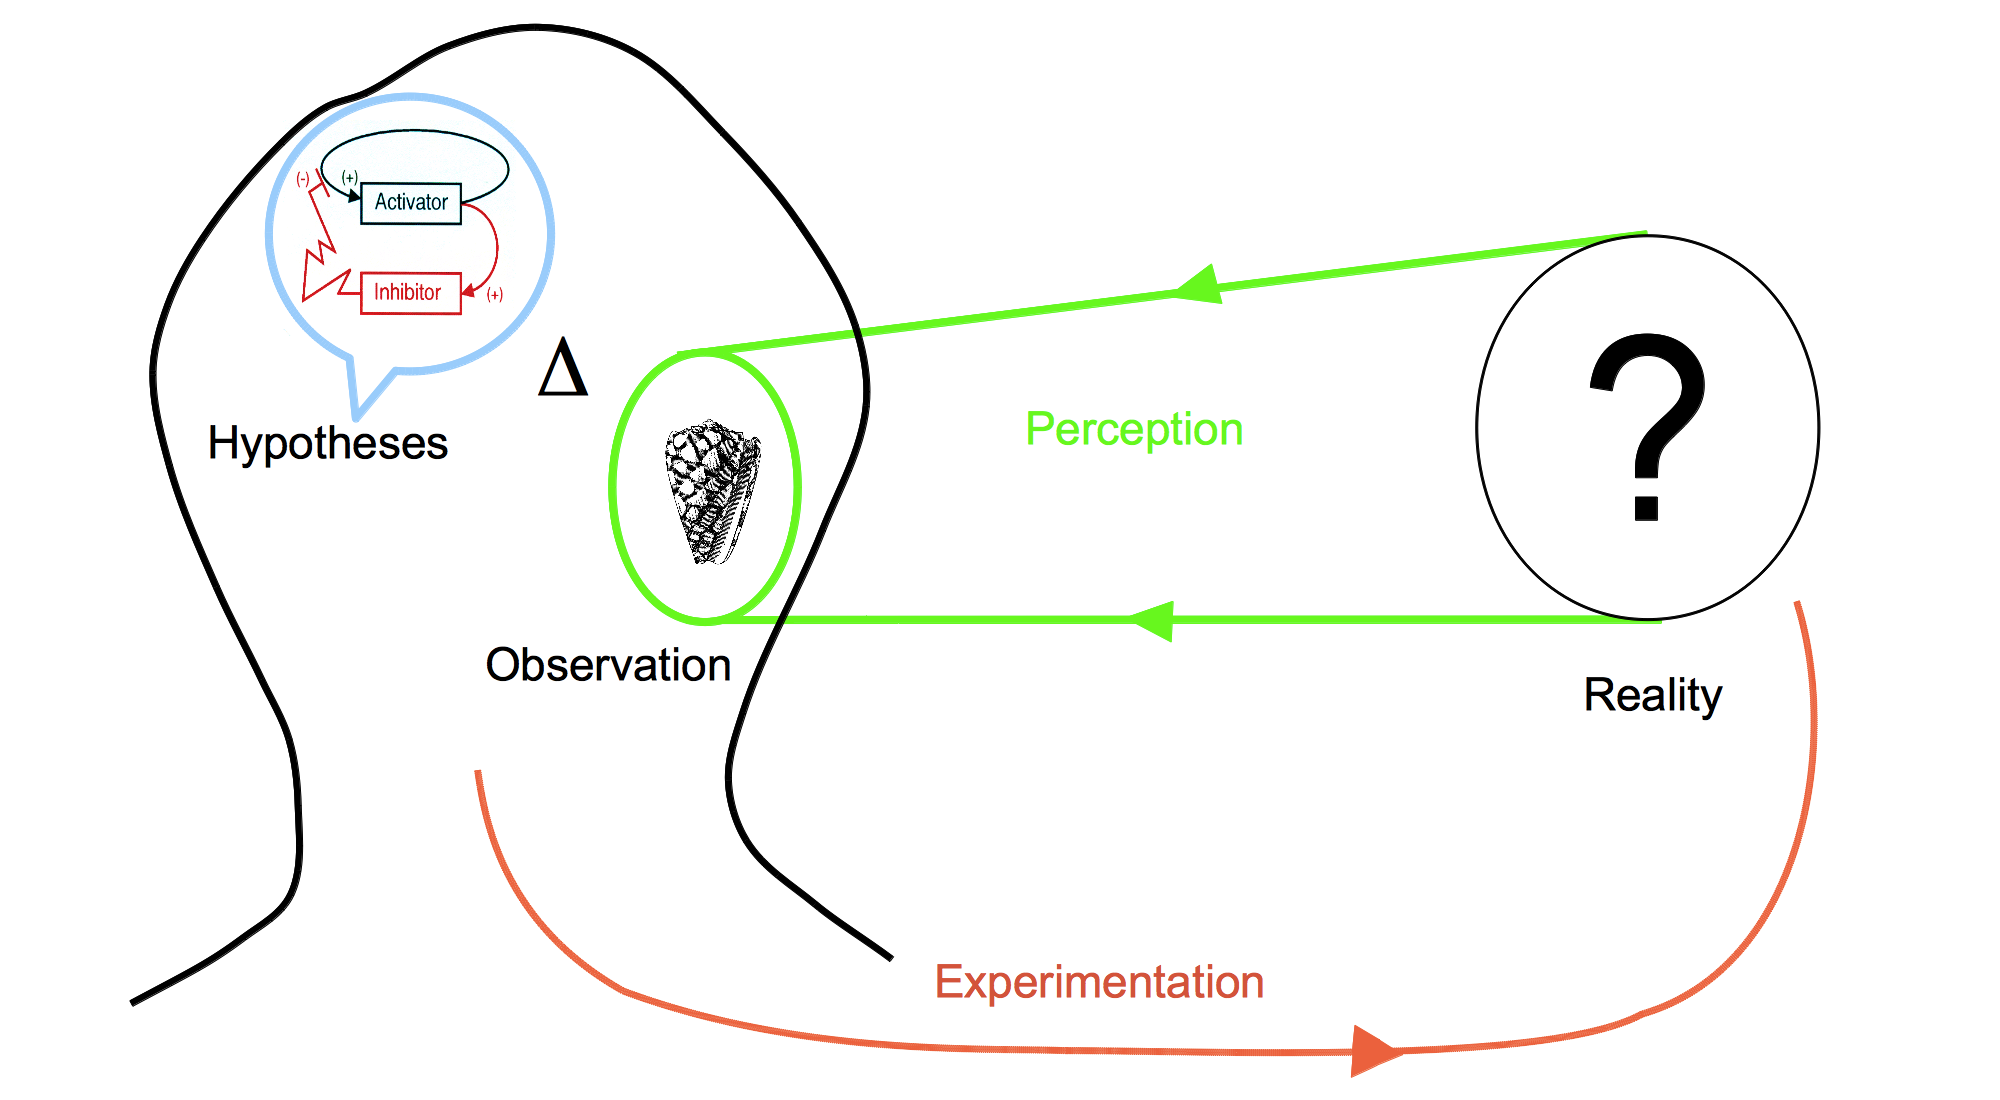
\includegraphics[width=0.95\textwidth]{../../images/experimental_science/experimental_science_raw_v2.png}
\end{center}
\caption{\textbf{The observation-hypothesis-experiment loop of experimental science. } It involves two main actors: the individual and reality (environment); and three main processes: perception, hypothesis generation (modeling), and experimentation.}
\label{experimental_science_schematic}
\end{figure}
\begin{enumerate}
	\item The loop can be entered by the individual perceiving and observing her/his environment.
	\item The observations made by this individual are then matched with the knowledge that s/he holds. Most of the time, observations conform to this knowledge and no particular reaction is elicited. Otherwise, a significant difference between the observations and what was initially expected by the observer triggers a "curiosity" signal that challenges her/his existing set of hypotheses and leads her/him to reconsider some of them. The cognitive processes by which s/he creates new hypotheses (e.g. analogy, inference, induction, abduction, or deduction) are not discussed here. Ultimately, "satisfying" hypotheses are the ones that can establish causal relationships among the observations. They can identify certain observations (the effects) as the consequences of others (the causes). Hypotheses also have a predictive value as they allow to extrapolate the behavior of the system when the causal factors are modified.
	\item The "experimental" qualifier attributed to many domains of biology or physics comes from combining the pure thought exercise of generating new hypotheses and real interactions with external objects in order to test the validity of these new hypotheses. The most efficient way for an observer-modeler to assess that the causal relationships that s/he inferred are compatible with her/his observations is to identify some elements of the studied object as potential "factors", then perturb these elements to modify the behavior of the studied object, and finally compare the new observed behavior with the predicted behavior. Note that the environment of the individual is made of multiple potential objects of study, so that the specification of one object of interest implies its separation from the environment, which may or may not include her/him. In developmental biology, the studied object is the embryo and the observer is excluded from the embryo's natural environment.
\end{enumerate}

\paragraph{Exchange/Validation by the Scientific Community}
%  ++++++++++++++++++++++++++++++++++++++++++++++++++++++++++++++++++++++ 


Even if the individual is at the center of experimental science, it is above all a \textit{collective} knowledge-building enterprise. The interaction between an observer-modeler and the rest of the scientific community operates bidirectionally (Fig. \ref{experimental_science_schematic_communauty}):
\begin{figure}
\begin{center}
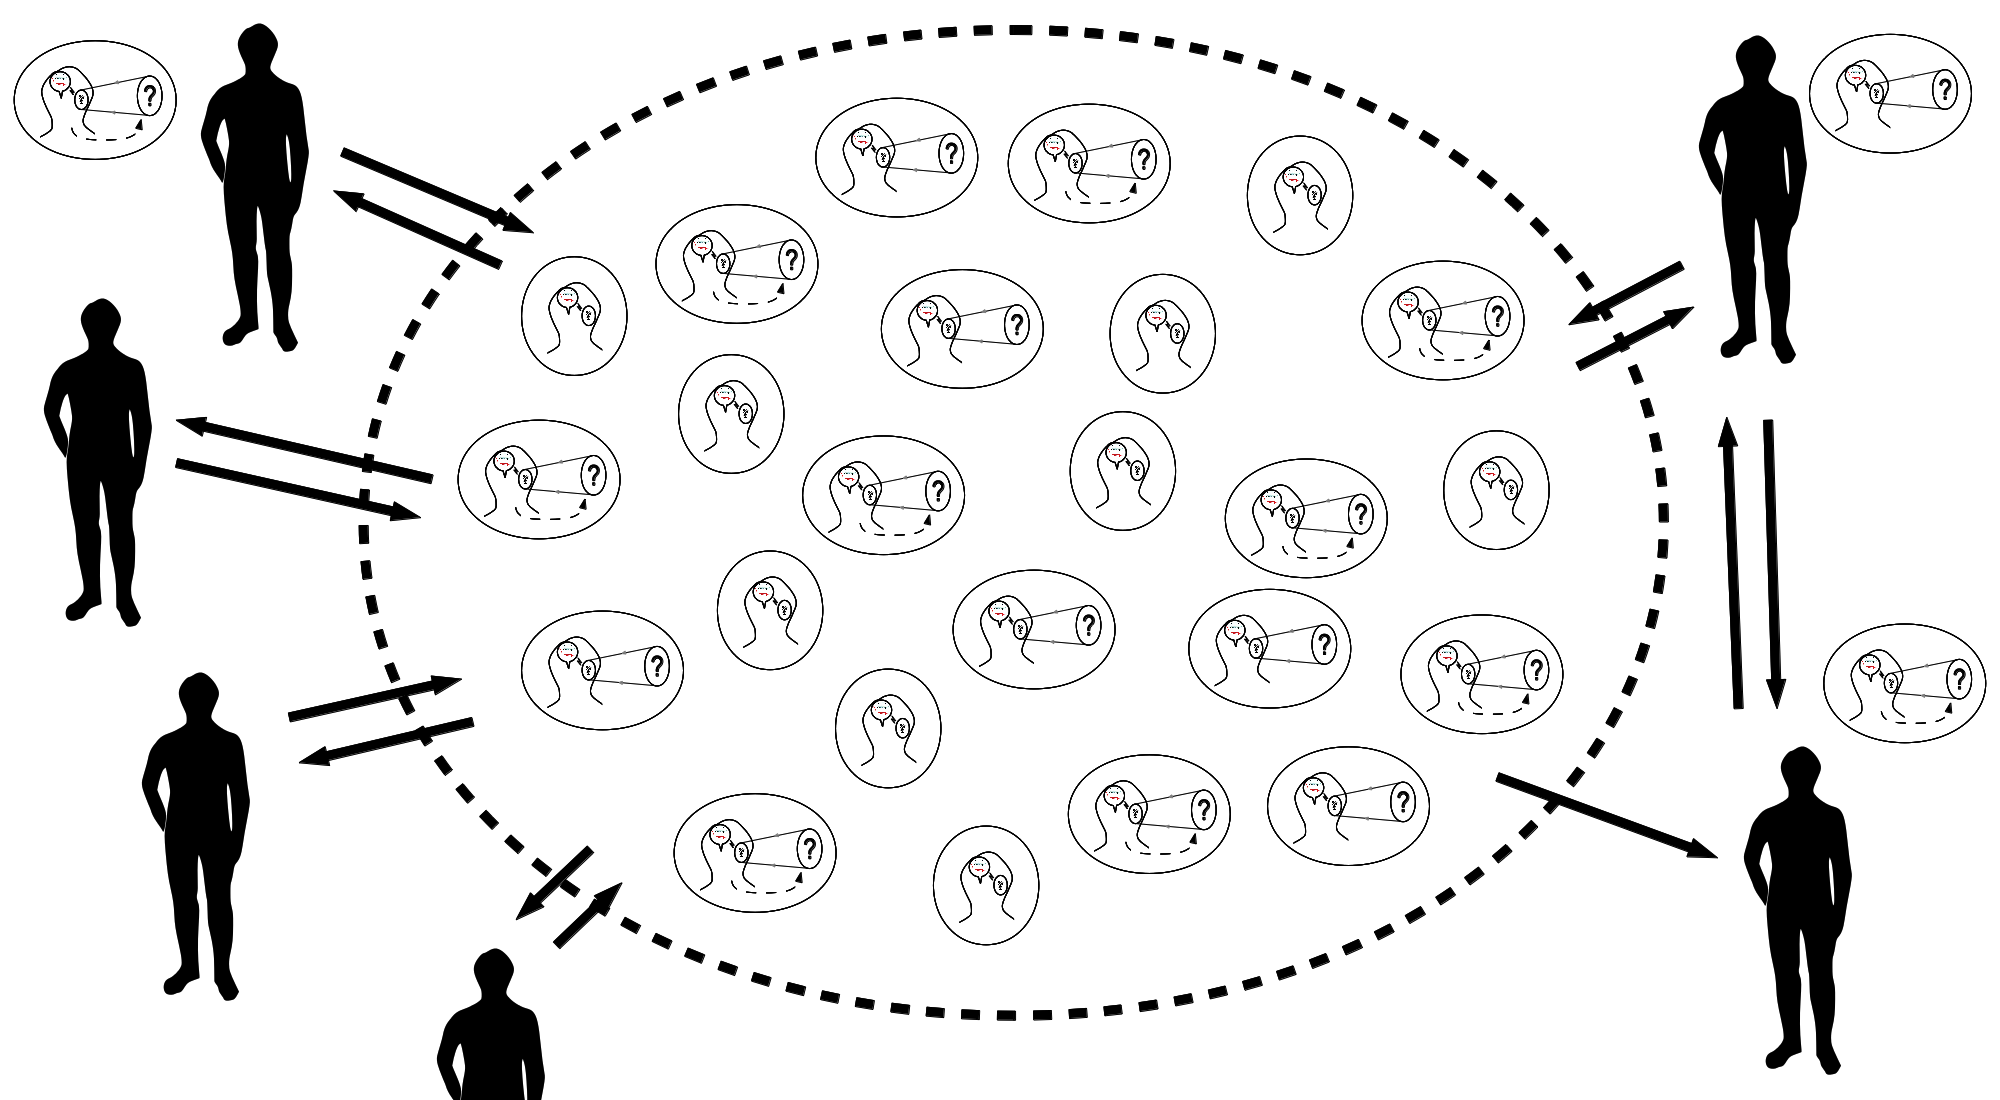
\includegraphics[width=0.95\textwidth]{../../images/experimental_science/experimental_science_communauty2.png}
\end{center}
\caption{\textbf{The collective effort of experimental science.} Each member of the scientific community may send or receive scientific work, which are verbal or written descriptions of parts or the whole observation-hypothesis-experiment loop.}
\label{experimental_science_schematic_communauty}
\end{figure}
\begin{itemize}
	\item All the hypotheses made by an individual are elaborated upon a historical accumulation of prior scientific works. Today, s/he is potentially able to access all of the knowledge produced by the scientific community thanks to Internet, in particular the various article databases (Pubmed, arXiv.org, IEEE, ACM, Google Scholar, etc.).
	\item One particularity of science is that the validation of a scientific work is ultimately decided by approval of the community. Through the peer-reviewed publication system, each new proposal is screened before being made available by a panel of individuals representing the community. This social dynamics is not without its problems, naturally (issues of motivation, expertise, time, politics, etc.), but consensus is basically the only mechanism that we have. We can distinguish between two types of peer validation: the \textit{validation of the scientific work} containing all or some parts of the elements illustrated in Fig. \ref{experimental_science_schematic}, and the \textit{validation of the hypotheses} contained in the scientific work itself. We will develop the latter aspect in Section 1.3.3.
\end{itemize}
%  ---------------------------------------------------------------------- 


\subsubsection{Designing Tools to Perceive, Conceive and Manipulate}
%  ---------------------------------------------------------------------- 


Experimental science insists on confronting hypotheses, the prediction they generate and observations. This confrontation is improved or "augmented" by the means of \textit{tools}. Tools can be considered the third actor in experimental science, in addition to the individual and the object of study. In fact, they are objects of study in themselves. In developmental biology, the technologies used to observe (microscopy) or perturb (genetics, chemistry, mechanics) a growing organism are the focus of intensive research in other fields of science. The advances of our understanding are closely coupled to the advances of these specialized and cutting-edge instruments. Microscopy imaging is constantly improving and expanding the spatiotemporal resolution and scope of observations. Every new microscope triggers a boom of new metholodogies, observations and conceptualizations. For example, Fig. \ref{experimental_science_perception_augmented} illustrates the perception pathway augmented with such tools. We examine below three types of tools designed to augment the three fundamental processes of experimental science: tools to perceive, tools to conceive, and tools to manipulate.

\paragraph{Tools to Perceive}
%  ++++++++++++++++++++++++++++++++++++++++++++++++++++++++++++++++++++++ 


Tools can greatly improve the perception of the studied object, whether upstream at the level of the interface between the real system and the observed (raw) data, or downstream at the level of the "reconstruction" and analysis of this data to extract salient features compatible with its interpretation. Perception-augmenting tools allow to reach information unaccessible to the natural senses of the individual: they widen the scope of perception and increase its resolution at the same time.

Perception-augmenting tools, however, can also perturb the natural behavior of the studied object by introducing external elements. For example, in the present study, microscope images are obtained by using artificially mutated specimens of fish or injecting fluorescent molecules, which are also heated by the laser light that is designed to illuminate them. Therefore, special care must be taken to evaluate, control, and maintain the possibly deleterious perturbation to a minimum.

The goal of perception-augmenting tools is to produce \textit{measures} of the studied object. Measures are a quantification of the physical attributes of the object by ordinary real numbers, the \textit{data}, which are scaled in "units". Therefore the data is the embodiment of the abstract notion of measure. Measures and data are never interpretation-free, as they are collected by choices that depend on prior knowledge. Thus their quantitative nature does not preclude subjectivity. They are indispensable resources that must be handled carefully and their scaling units validated by consensual agreement.
\begin{figure}
\begin{center}
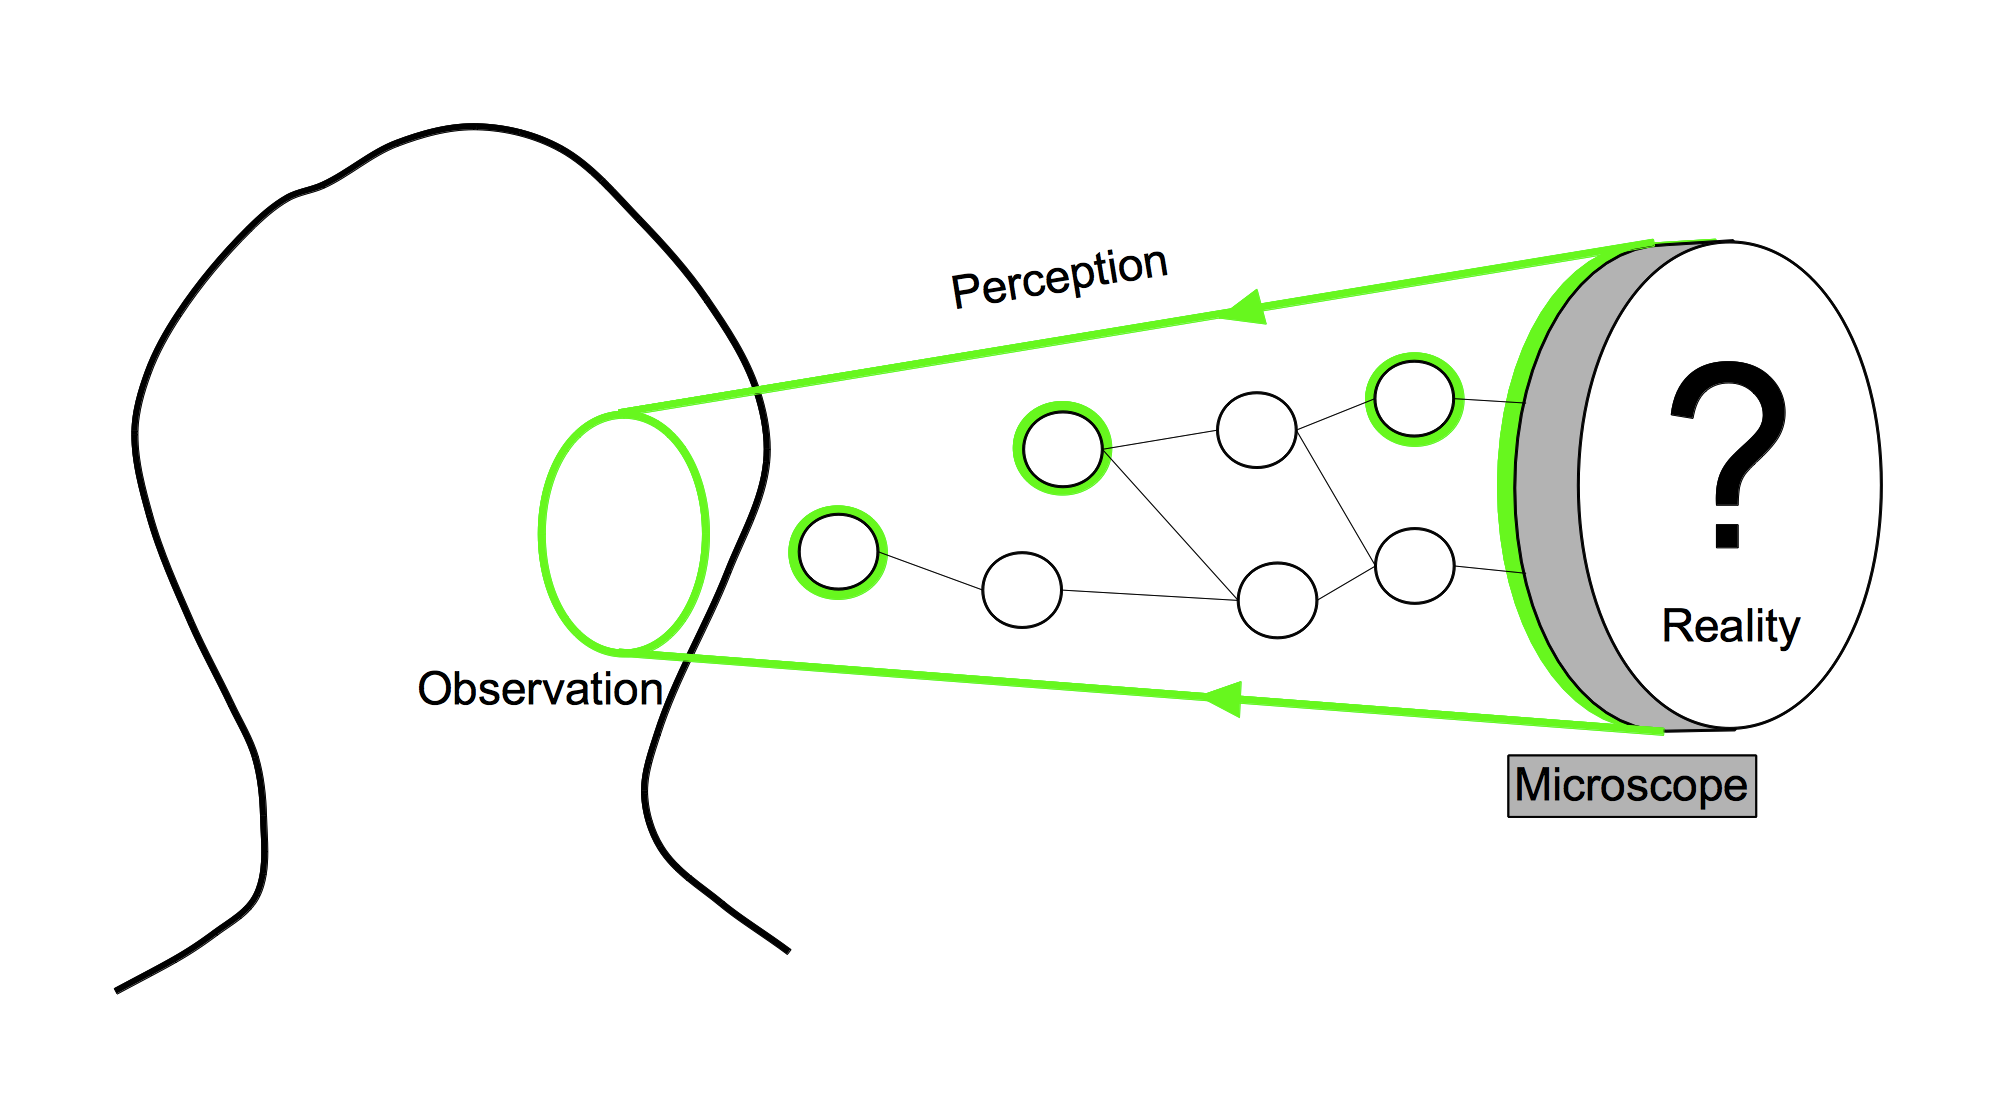
\includegraphics[width=0.95\textwidth]{../../images/experimental_science/experimental_science_perception_augmented2.png}
\end{center}
\caption{\textbf{Augmented perception with interfacing tool (optical microscope) and a reconstruction workflow.}}
\label{experimental_science_perception_augmented}
\end{figure}

\subparagraph{Optical Microscopy: An Interface with the Studied Object}
%  ........................................................ 


In developmental biology, the principal perception-augmenting tools are obviously optical microscopes. The sets of measures used in the present project are originating from these devices. Other tools used in developmental biology, but more disruptive ones, are force microscopes and molecular biology techniques such as DNA/RNA microarrays, and macromolecule blotting and probing.

Optical microscopes extend our natural perception to the cellular scale and below. The general principle is to send photons to excite small regions of the embryos, which in turn emit other photons that are collected by camera sensors through objective lenses. The path of the exciting light beam can be controlled to cross the region of interest in the embryo. A software automates the task and automatically associates the spatial coordinates of the excited region to the quantity of photons captured by the sensors. An extensive scan produces a certain volume of "voxels" (3D pixels) that store the spatially localized quantity of photons emitted by the embryo. This process is repeated multiple times and a time-series of 3D volumes is generated, eventually producing 4D (or "3D+t") \textit{raw data}.

The value stored in a single voxel is called its intensity and belongs to a first category of raw data that we call here \textit{local microscopic measures}, which are characterized by the smallest resolution both spatially and temporally. Then, the aggregation of all these local measures produces \textit{extensive local measures}, a second category of raw data that can otherwise be called a "field" and contains the complete set of information captured by our perception-oriented device. Raw data presents two challenges:
\begin{itemize}
	\item Its size is generally enormous. A few hours of embryonic development under the microscope typically produces billions of integer values. For example, 200 3D volumes of voxels of intensity sampled every 3 minutes, each volume having a resolution of $512 \times 512 \times 200$ yields over $10^{10}$ values. This size may can also be multiplied by the number of channels used for light excitation. In the present study, two different channels are used for nucleus and cell membrane labeling. Multiple channels can be used to capture the light emitted by fluorophores that label gene expression \cite{Ducros:2011km}.
	\item Consequently, profuse raw data is abstruse: it cannot be interpreted easily and no biological insight can be gained from direct observation.
\end{itemize}

\subparagraph{Phenomenological Reconstruction }
%  ................................ 


Computers offer visualization software tools that allow the observer-modeler to create 3D+t movies of the captured developmental sequences. While a raw movie can certainly lead to qualitative insights, it also critically lacks quantitative measurements. Thus data \textit{processing} is a necessary step toward a comparison with the predictions derived from the hypotheses, and a final interpretation. Here, we call this step the \textit{phenomenological reconstruction}, or simply "reconstruction", of the data. The idea is that, since raw data contains more or less incomplete information on the structure of the imaged embryos, depending on the spatiotemporal resolution and signal-to-noise ratio of the microscope, missing pieces have to be quite literally "reconstructed". Moreover, as the reconstruction is realized from prior knowledge about the studied object, which is subjective with respect to the individual, this reconstruction is also "phenomenological".

The reconstruction process is composed of a series of subprocesses organized in a \textit{workflow}. Each subprocess carries out a specific task that extracts some information from the input data sets, completes it, and generates new data sets (Fig. \ref{schema_raw_reconstructed_embryo_macroscopic}). The question is then to define what type of measure the phenomenological reconstruction is aimed at. As described in Section 1.1, the individual cell's dynamics is the fundamental unit of comprehension of biological development. The objective is thus to reconstruct the collective spatiotemporal dynamics of all cells taken together. The format we propose to use here is organized around the \textit{lineage tree}, which follows along a global time line the complete cell genealogy starting from the zygote (Fig. \ref{schema_raw_reconstructed_embryo_macroscopic}). Each item of this graph represents a cell at a given time step. As we progress along the time axis, each item is connected downstream (a) either to a single item representing the same cell at the next time step, (b) or to two items if the cell has divided, where each item represents the daughter cells. The lineage tree is then enhanced or "decorated" by labeling each item with local observations about the cell it represents, describing its dynamics: its spatial 3D coordinates, membrane shape, list of neighbor cells, and various scalar quantities representing the fluorescent labeling molecules (RNA, proteins, etc.). In future work, we plan to add more precise information about asymmetrical quantities of labeled molecules, which represent cell polarity.
\begin{figure}
\begin{center}
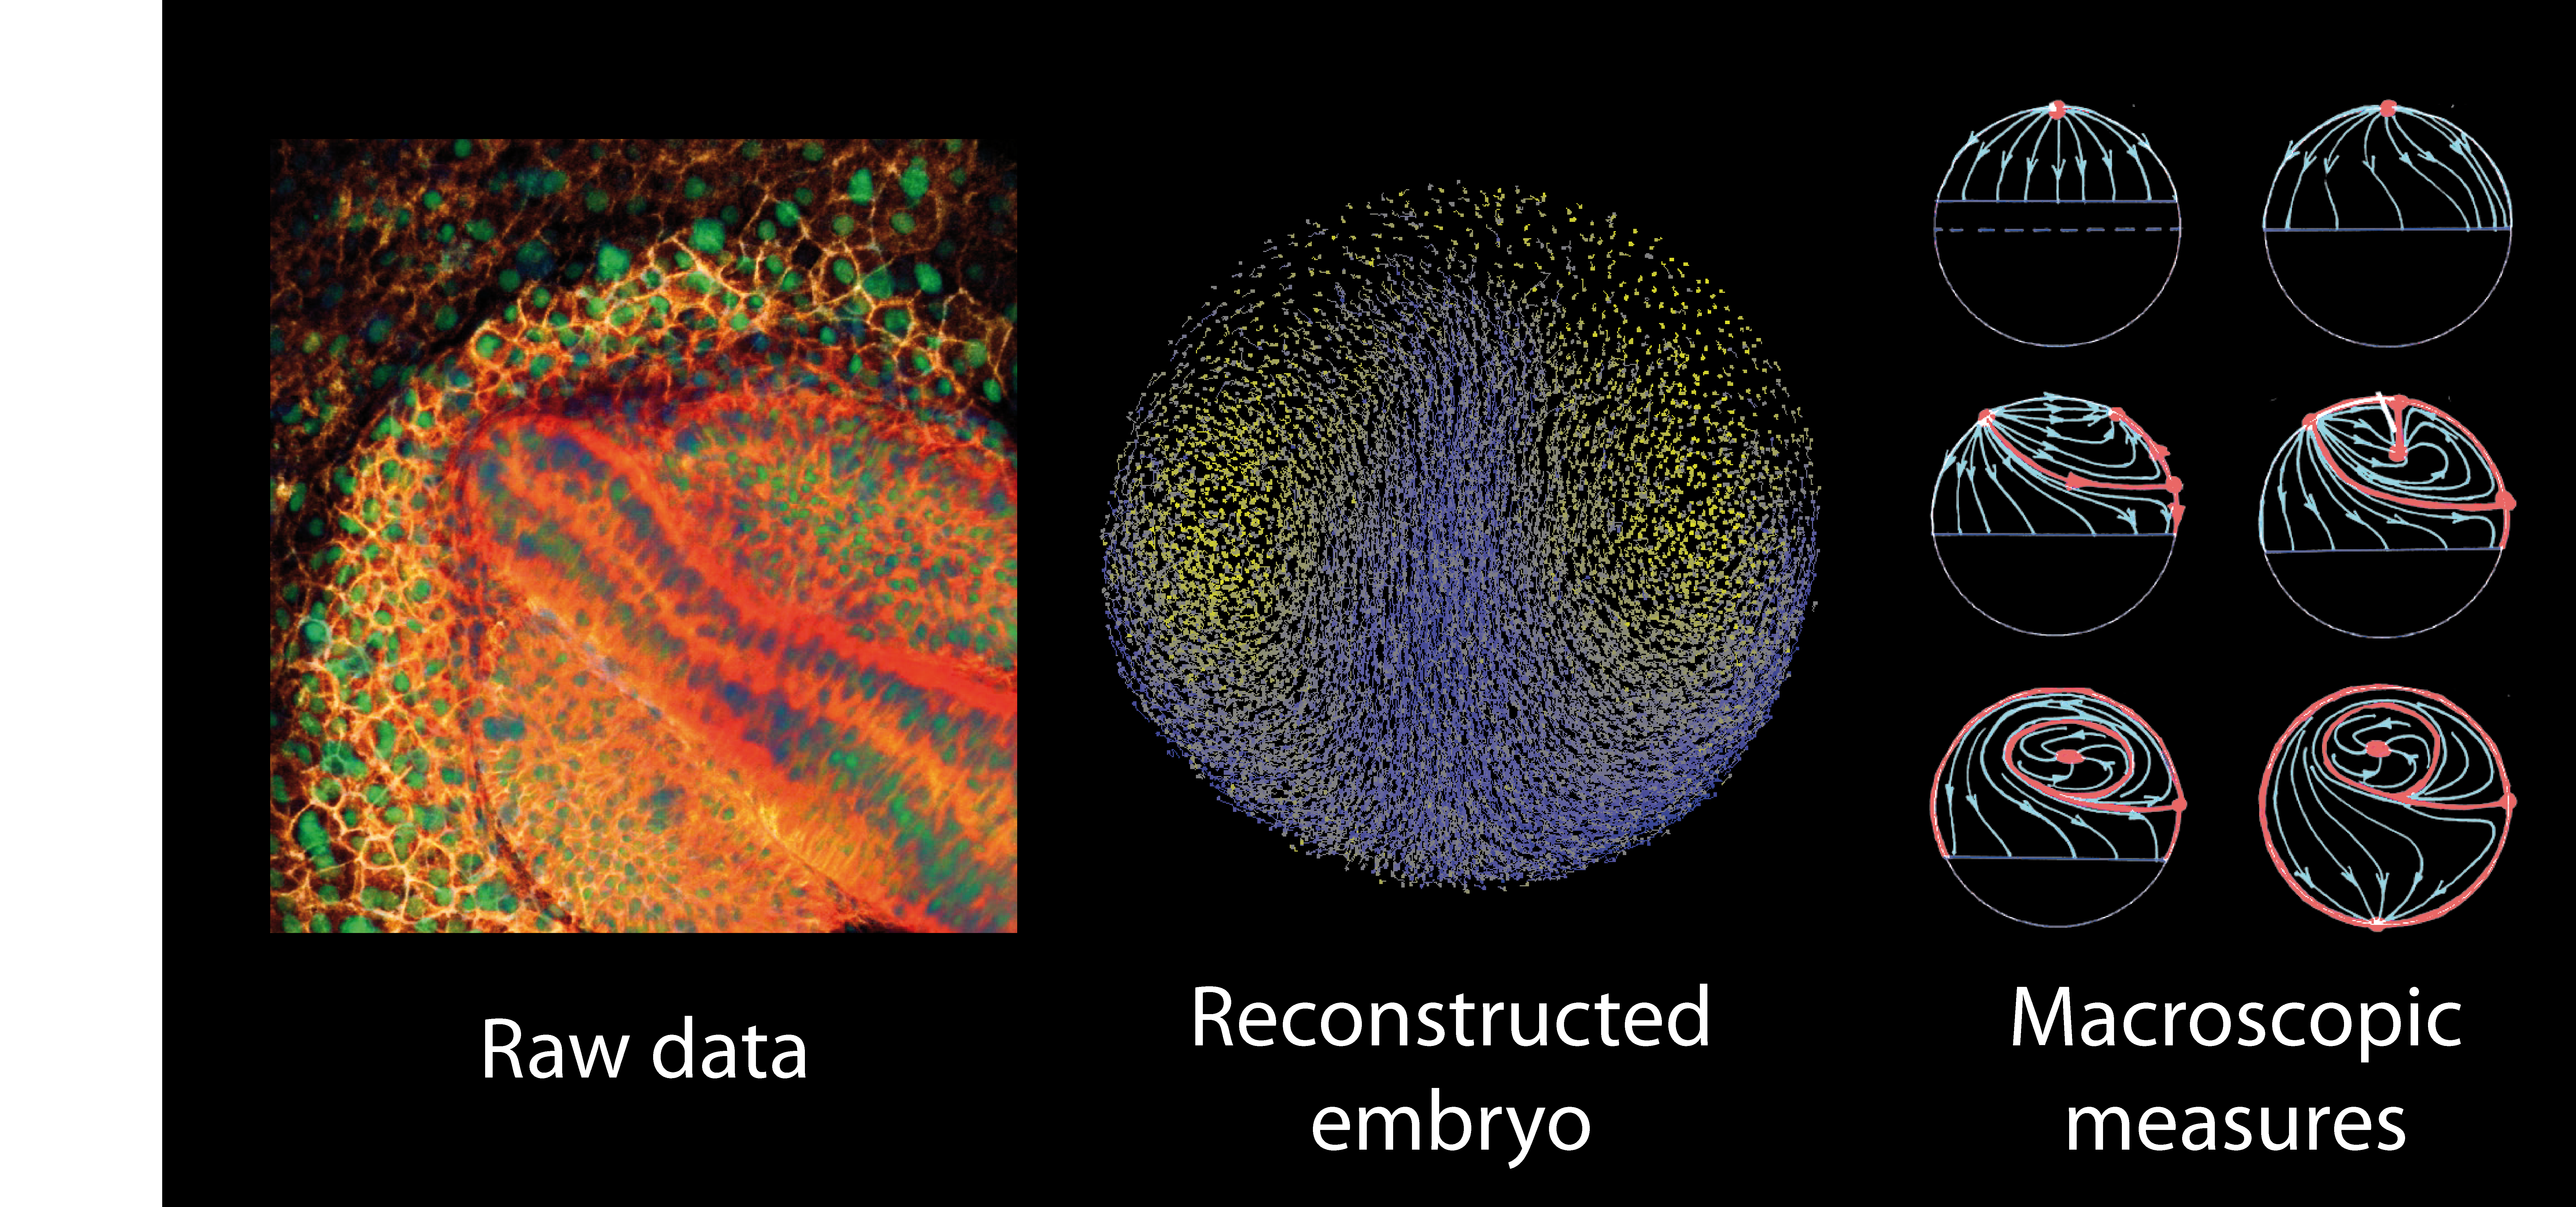
\includegraphics[width=0.95\textwidth]{../../images/experimental_science/schema_raw_reconstructed_embryo_macroscopic.png}
\end{center}
\caption{\textbf{The three major steps of the reconstruction in the BioEmergences platform: raw data, reconstructed embryo and macroscopic measures. } Left: raw data of the zebrafish developing head (nuclei labeled in green and cell membrane in red). Center: visualization of the reconstructed embryo with the MoveIt software. Small dots are the cell centers and arrows gives the future cell displacement. Colors indicates the velocities of the cell. The central image illustrates the extremely high dimensionality of the reconstructed embryo. Right: Macroscopic measures of the displacement field in the developing embryo (from B. Lombardot PhD manuscript \cite{Lombardot:2010vd}. Images realized by the BioEmergences team.}
\label{schema_raw_reconstructed_embryo_macroscopic}
\end{figure}

Equipped with this enhanced lineage tree, which we call the \textit{reconstructed embryo}, the cell dynamics can be followed through space and time. The structured format of this exhaustive set of measurements allows comparison with predictions from the hypotheses, and among different reconstructed specimens. The reconstructed embryo is an "extensive local measure", following the term we defined earlier. While it greatly facilitates and accelerates the handling of observations, the problem is that its dimensionality is also huge---as it scales with the number of time steps multiplied by the number of cells per time step multiplied by the number of local measures per cell. Thus it represents only the foundation of a higher level reconstruction of the embryo dynamics, which ultimately provides the individual with interpretable biological facts. This higher level reconstruction represents a third category of data, which we call \textit{macroscopic measures}. The macroscopic measures are obtained by projecting the enhanced lineage tree space onto specific low dimensional space characterizing biological properties. Performing multiple macroscopic measures allows a relevant characterization of the behavior of the global dynamics of the developing embryo.

Some of the reconstruction modules can be realized with off-the-shelf commercial software. However, the high number of cells involved and the difficulty to interpret and manipulate the 3D volume of data initiated in our group the design and implementation of better suited custom software and greater automation of the workflow of these subprocesses. Nadine Peyri\'eras at the NED (formerly DEPSN) in Gif-sur-Yvette and Paul Bourgine at the CREA lab and ISC-PIF institute in Paris, spearheaded two major European projects gathering several teams in six different countries: \textit{Embryomics} (ended in 2009) and \textit{Bioemergences} (renewed), which pioneered the design of such reconstruction methods and algorithms. While the biologists of the group produced and annotated time-lapse series of organism development, the mathematicians and computer scientists processed these images through specialized algorithms and transformations such as filtering, segmentation, detection, and tracking. This effort resulted in sophisticated software \textit{"platforms"} capable of handling large amounts of 4D voxel movies of vertebrate embryos, and producing in output partial or complete cell lineage trees (see Chapter 7). For our part, we added new modules that we designed and implemented specifically for the present study. A detailed presentation of these workflows and our own contribution will be found in Chapter 7.

\paragraph{Tools to Conceive}
%  ++++++++++++++++++++++++++++++++++++++++++++++++++++++++++++++++++++++ 


Cognitive scientist Marvin Minsky provided a general definition of a model in his 1965 article \textit{Matter, mind and models}\cite{Minsky:1965wb}: \textit{"To an observer B, an object A* is a model of an object A to the extent that B can use A* to answer questions that interest him about A".} This definition is centered around the notion of "question" asked by the observer. The model is an object whose raison d'être is to satisfy its designer and, eventually, others around her/him. In this section, we discuss the nature of theoretical models, and particularly causal models. We believe that tools are also able to augment the capacity of the individual to make and test hypotheses, by providing interactions with a model that push her/him beyond her/his usual reasoning abilities.

\subparagraph{Means of Expression}
%  ................... 


Models are constrained by their means of expression. The descriptive power of the structures and their interactions can vary greatly depending on whether they are expressed verbally, graphically or mathematically. Models are often described through a combination of the above. In the context of developmental biology, a distinction is often made between "classical" studies and "theoretical" studies: generally, the former use verbal and graphical formalism, while the latter use mathematical formalism.

\subparagraph{Mathematical Formalism}
%  ...................... 


In the mathematical formalism, objects are represented by variables, and their interactions are put into functions or equations. Generally, this formalism is expressed in "analytical form" using basic arithmetic operations such as $+$,$-$,$\times$,$\div$), power, exponential, logarithm, or infinite times series. In experimental science, the quantities involved tend to vary temporally and/or spatially, and their rates or derivatives play an important role. Typically, "ordinary differential equations" (ODEs) for time-varying quantities only or "partial differential equations" (PDEs) for time and space-varying quantities are used.

\subparagraph{Dynamical Systems}
%  ................. 


In classical mechanics derived from the Newtonian laws, the time variable $t$ holds a particular status. It is considered an "absolute", meaning that two events are temporally separated by the same interval for all observers. This assertion is not correct in relativistic physics, where the notions of space and time are intermingled. However, the classical mechanics assumptions have founded a theoretical framework that produced accurate results for systems where objects are moving at a speed much smaller than the speed of light, or have sizes much larger than the atomic or sub-atomic scale (the realm of quantum mechanics)---which is obviously the case of all models of developmental biology discussed in the present work. Therefore, in the case of growing embryos that undergo spatiotemporal transformations, all theoretical representations fit well in the classical paradigm of \textit{dynamical systems}. A dynamical system is built from three elements:
\begin{itemize}
	\item the \textit{state space}: the state of a modeled system being a collection of variable at a given time, the state space encompasses all the possible states that the system can adopt; it is defined a priori
	\item a set of equations that determine the laws of evolution of the system
	\item the initial state, i.e. the state of the system at the initial time from which the dynmical system evolves.
\end{itemize}

The interest of the dynamical system paradigm is that it does not restrict a model to a particular set of equations, but makes the space of possible values that variables can take and their initial conditions an important part of the hypotheses that define a model. Dynamical systems can be deterministic or stochastic if a random term (such as noise) is used in the differential equations. In a deterministic model, a state at any given time entirely determines a unique trajectory of future states of the system (Fig. \ref{experimental_science_multi_initialstate}).

\subparagraph{Parameters}
%  .......... 


Certain variables have a special status as they are, by hypothesis, intended to remain constant along the state trajectories. In that case, they are called \textit{parameters}. The design of a model must deal with parameters as much as with the mathematical laws of evolution. Selecting the parameters among the variables depends on the use of a model. Depending on the context, some parameters may be always fixed at a specific values because they have been confirmed by direct experimental measures. Parameters generally have their own space, the \textit{parameter space}. Each point in the parameter space can be associated with a state trajectory (Fig. \ref{experimental_science_multi_initialstate}).
\begin{figure}
\begin{center}
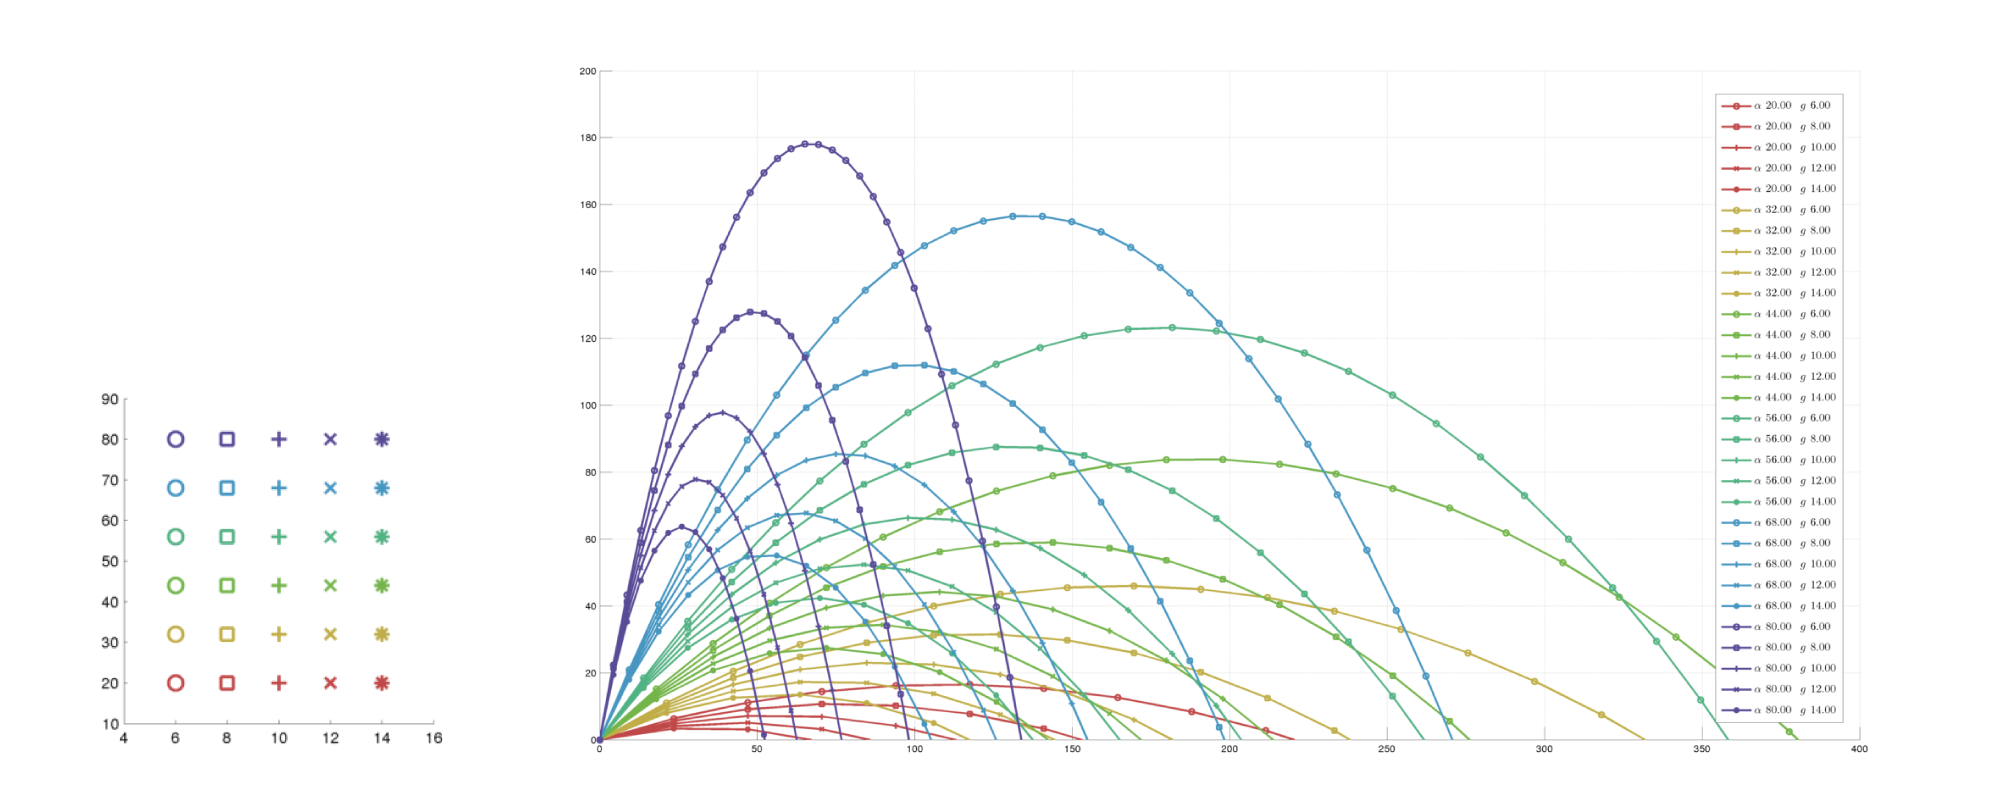
\includegraphics[width=0.9\textwidth]{../../images/experimental_science/multi_initialstate_fusion.png}
\end{center}
\caption{Simple illustration of a dynamical system: if a ball is hit by an object, it will move in space following a parabolic curve until it lands on the ground. A classical mechanics model would consider the curve (i.e. the temporal evolution of the position) as the "phenotype", which is determined only from an initial known position and the velocity of the ball. Left: parameter space, Right: phenotypic space.}
\label{experimental_science_multi_initialstate}
\end{figure}

During the study of a model, a parameter may reveal itself as non-constant (we never "know" if a parameter is truly constant, see validation section below). The reaction is to hypothesize a new rule for the evolution of the parameter and add it to the mathematical set of rule. This operation is a common part of the building of model.

\subparagraph{Theoretical Models, Analytical vs. Computer-Simulated Models}
%  ............................................................ 


As mentioned above, theoretical models formalize the interactions among the system with equations that link together some of the selected variables of the studied phenomenon. Solving this \textit{analytical} formalism is not always feasible because of constraints that are specific to mathematical symbolic transformations. Computers can help in this situation by converting equations into algorithms and calculating \textit{numerical} solutions, which are approximations of the ideal solutions. Used nowadays in every field of research and engineering, numerical analysis allows scientists to tackle more complex phenomena. In 1952, Alan Turing already envisioned the use of computer to help him solve more realistic reaction-diffusion patterns in "The chemical basis of morphogenesis":
\begin{quotation}  Most of an organism, most of the time, is developing from one pattern into another, rather than from homogeneity into a pattern. One would like to be able to follow this more general process mathematically also. The difficulties are, however, such that one cannot hope to have any very embracing theory of such processes, beyond the statement of the equations. It might be possible, however, to treat a few particular cases in detail with the aid of a digital computer. This method has the advantage that it is not so necessary to make simplifying assumptions as it is when doing a more theoretical type of analysis \cite{Turing:1952vn}. 
\end{quotation}

Turing emphasizes the fact that the use of computer simulation is not only a practical solution to treat analytically unsolvable mathematical equations, but also that it allows the individual to integrate new mechanisms that s/he would refrain from using because of their mathematical unsolvability. In this sense, the computer (as a Turing machine) is a tool that augments the ability of the individual to develop mathematical models of the object of study.
\begin{figure}
\begin{center}
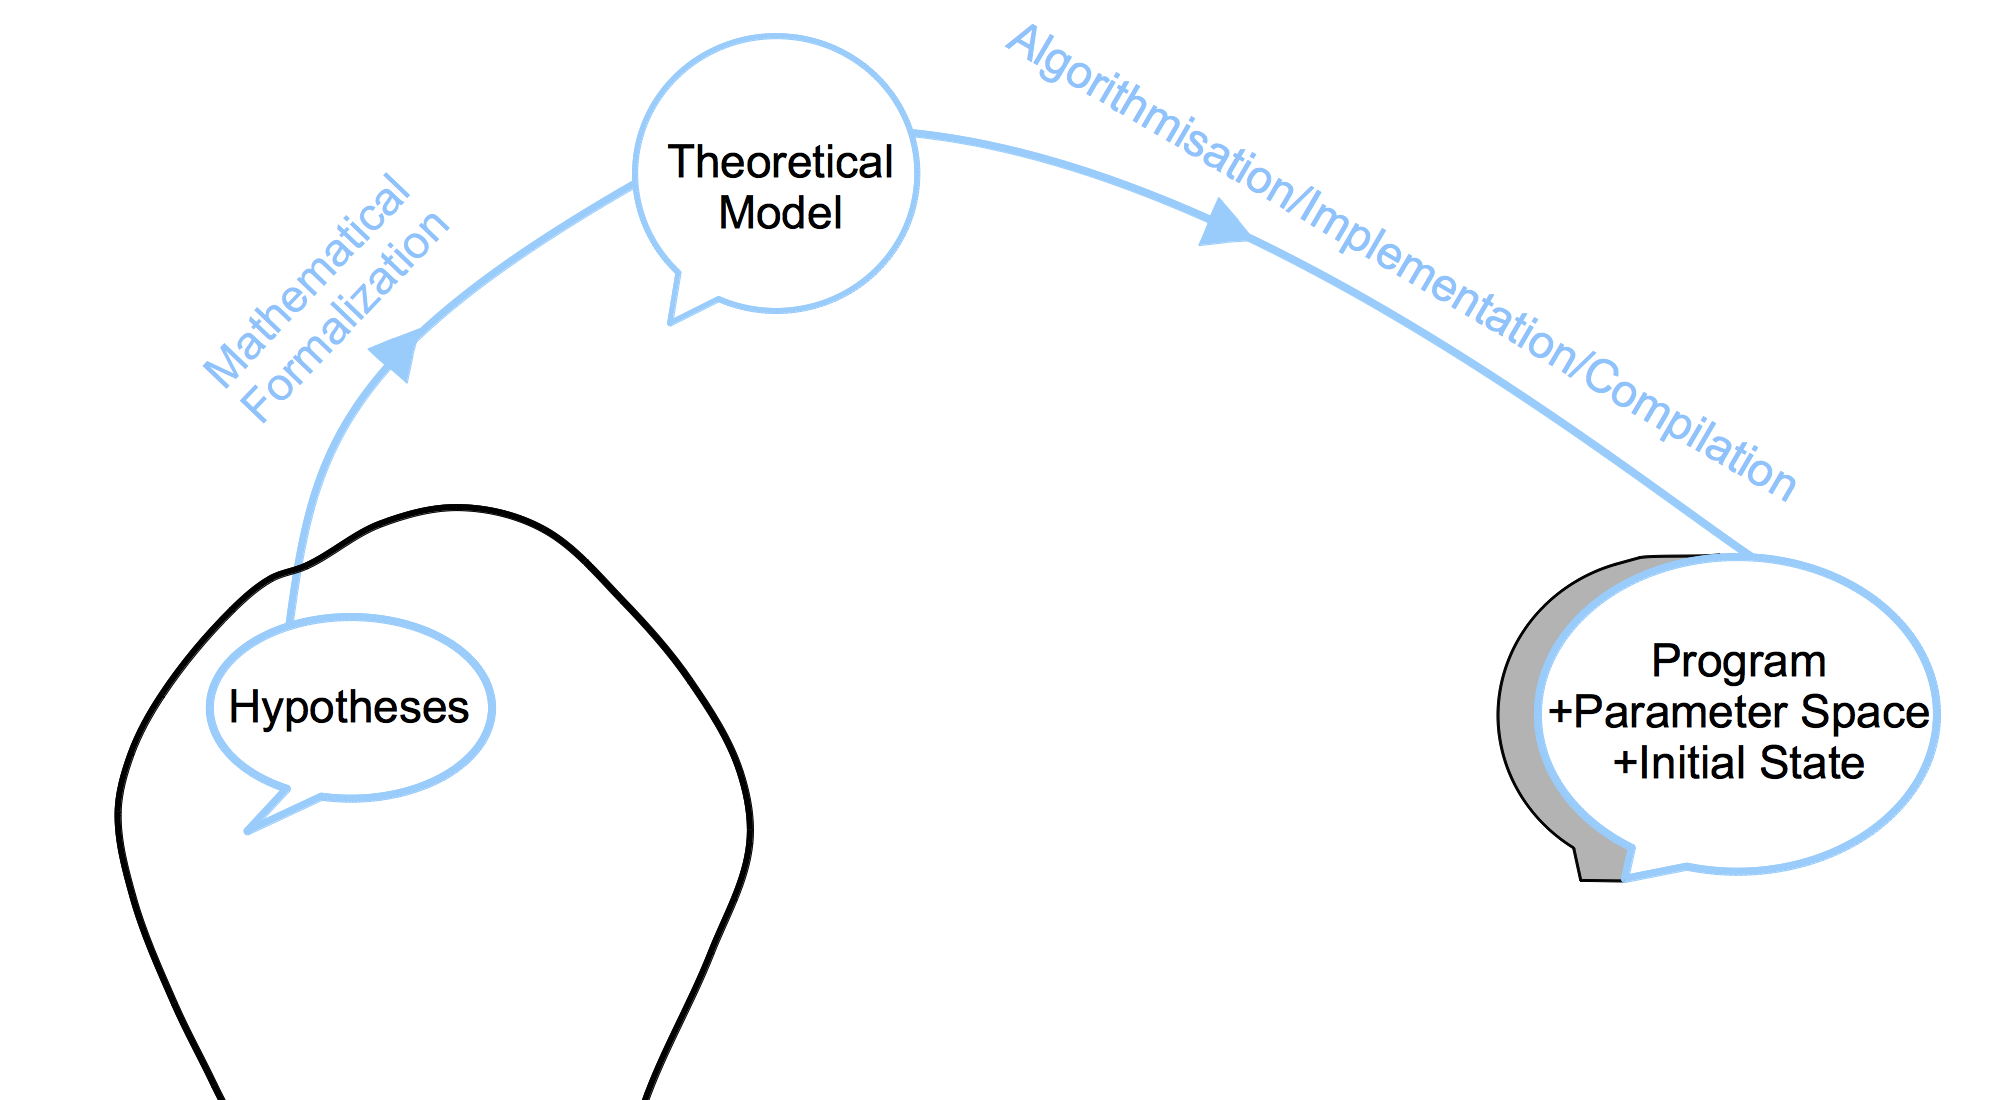
\includegraphics[width=0.95\textwidth]{../../images/experimental_science/experimental_science_hypotheses_augmented2.png}
\end{center}
\caption{\textbf{Augmentation of hypothesis generation through theoretical model and computer simulation.}}
\label{experimental_science_hypotheses_augmented}
\end{figure}

An important category of analytically unsolvable models are called \textit{many-body problems}, which concern most complex systems. They occur when a large number of elements are interacting together. As we will present in Chapter 3, the physical approach that we have chosen for our embryogenesis model is based on this assumption, each cell being an elementary particle interacting with its neighbors. Solving this system of equations is highly computationally intensive and requires the use of many computing units in parallel, such as computer clusters or graphical processing untis (GPUs). In fact, computers were originally invented to deal with theses situations (for example, the MonteCarlo simulation performed on the MANIAC computers in the early 1950's \cite{Metropolis:1987ws}). Figure \ref{experimental_science_hypotheses_augmented} illustrates the process of transformation of the model, from the original hypotheses made by the individual, to its theoretical form, and finally to its final form as a computer program.

\subparagraph{"Black Box" Models}
%  .................. 


The type of models that have been considered so far are what some would call "white box" models: they are elaborated from specific hypotheses, and try to provide a mechanistic explanation. In contrast, "black box" models are empirical models built without a priori knowledge. These data-driven models are essentially \textit{statistical} and used for data mining purposes. In our study, we have ruled out this category as they do not follow the framework of individual-induced hypotheses described above. Black-box models certainly possess predictive capabailities but they have little or no explanatory value, since the internal rules that they form are not directly interpretable. To tis category belongs machine learning, such as neural networks or support vector machines, and evolutionary computation. An intermediary category, "gray box" models may be defined if partial knowledge of the system is included in the black box.

In conclusion of this section, as stated by Turing when introducing his reaction-diffusion model, a model is a "simplification and an idealization, and consequently a falsification" \cite{Turing:1952vn}. This description applies to all models, whether theoretical or "classical", but mathematical formalism obviously still plays a fundamental role in at least three ways:
\begin{itemize}
	\item Predictability: theoretical models allow to test hypotheses and postulate the behavior of complex systems in a way that "pure thought" could not. They are not a replacement for the experimental part, but they can perform theoretical pre-experiments to specify the conditions of "real" experiments.
	\item Abstraction: the idealization process allows to simplify the hypotheses and determine which mechanism is essential and which one is not.
	\item Precision: however sensitive qualitative transitions between different regimes or behaviors of a system may be, mathematical formalism can be adapted to any scale.
\end{itemize}

\paragraph{Tools to Manipulate}
%  ++++++++++++++++++++++++++++++++++++++++++++++++++++++++++++++++++++++ 


A third category of tools were designed to interfere with and modify the "natural" behavior of the objects of study, or their environment, in a controlled manner. Such experiments are artificial constructions that are designed to discriminate and select among various hypotheses about the rules of behavior of a system. In developmental biology, the embryo can be perturbed in two major ways: genetically or mechanically. Genetic experiments consist in making the embryo express an abnormal phenotype, either by random mutagenesis or by "morpholino" injection (specific gene knock-out). Mechanical experiments can be done either through a lesion applied to a specific tissue to study its fate (e.g. laser ablation between individual cell-cell boundaries \cite{FernandezGonzalez:2009hp}\cite{Landsberg:2009bp}, and tissue dissection by laser \cite{Behrndt:2012gy}), or by some mechanical constraint to measure the response of the tissue. "Mechanotranduction" mechanisms also allow to conceive experiments at the interface between genetics and mechanics, such as provoking new genetic regulation by exerting a force with magnetic tweezers or magnetic nanoparticles \cite{Desprat:2008ei}).

As it will be discussed in Section 2.2, studying an object often begins with studying its parts. In developmental biology, \textit{in vitro} experiments allow to isolate cells or tissue, and test their behavior under controlled conditions (e.g. cell sorting experiments). One pitfall of this approach can be underestimating the impact of the artificial conditions on the behavior of the part, compared to its usual \textit{in vivo} conditions. This can lead to the design of more complete in vitro environments that try to mimic and recreate the natural cellular "habitat", as is the case for stem cells \cite{Nishikawa:2007jl}.
%  ---------------------------------------------------------------------- 


\subsubsection{Reality Check: Validating the Hypotheses}
%  ---------------------------------------------------------------------- 


The concept of \textit{validation} of a hypothesis, which is employed in this work, can not be understood in the same sense as stating that an hypothesis is definitively true or false. Oreskes \cite{Oreskes:1994gn} has demonstrated that establishing the truth of a proposition is possible only in a closed system, and that models using incompletely known input parameters as is the case in developmental biology are never closed systems. Popper \cite{Popper:1959uo} also advocates that one cannot "prove" theories and laws, and that they can only be "falsified". Thus in our case, "validation" can only mean a certain degree of \textit{consistency} between the output of the model and the observations made about the object of study. Observations can support the likelihood of a model \cite{Oreskes:1994gn}, or its empirical adequacy \cite{vanFraassen:1980uy}.

The goal of an explanatory model is not merely to reproduce observations (as in the black-box methods) but rather unravel the principles that are at the foundation of these observations. The more observed data are positively confronted to the model, the more "adequate" the model and its underlying principles are deemed. The diversity of the observed data is another factor in favor of the adequacy of the model. A framework must also be designed to practice and confront the model against the observations of the studied phenomenon. The strategy that we adopt here is to \textit{integrate the simulation platform and the reconstruction workflow}. In the same way that a microscope produces "real raw data", our program generates "simulated raw data". Then, the same reconstruction step is applied to both branches in parallel, giving rise to "reconstructed real data" and "reconstructed simulated data" (where reconstruction may refer to local microscopic, extensive microscopic or global mesures; see above), which are later compared to each other. The reconstruction workflow gets a new leg from the theoretical process of our general experimental science scheme (Fig. \ref{experimental_science_larger_augmented}). The different natures of the simulated and experimental data require that reconstruction algorithmic modules be applied so that they can be compared based upon the same format and automatically processed.
\begin{figure}
\begin{center}
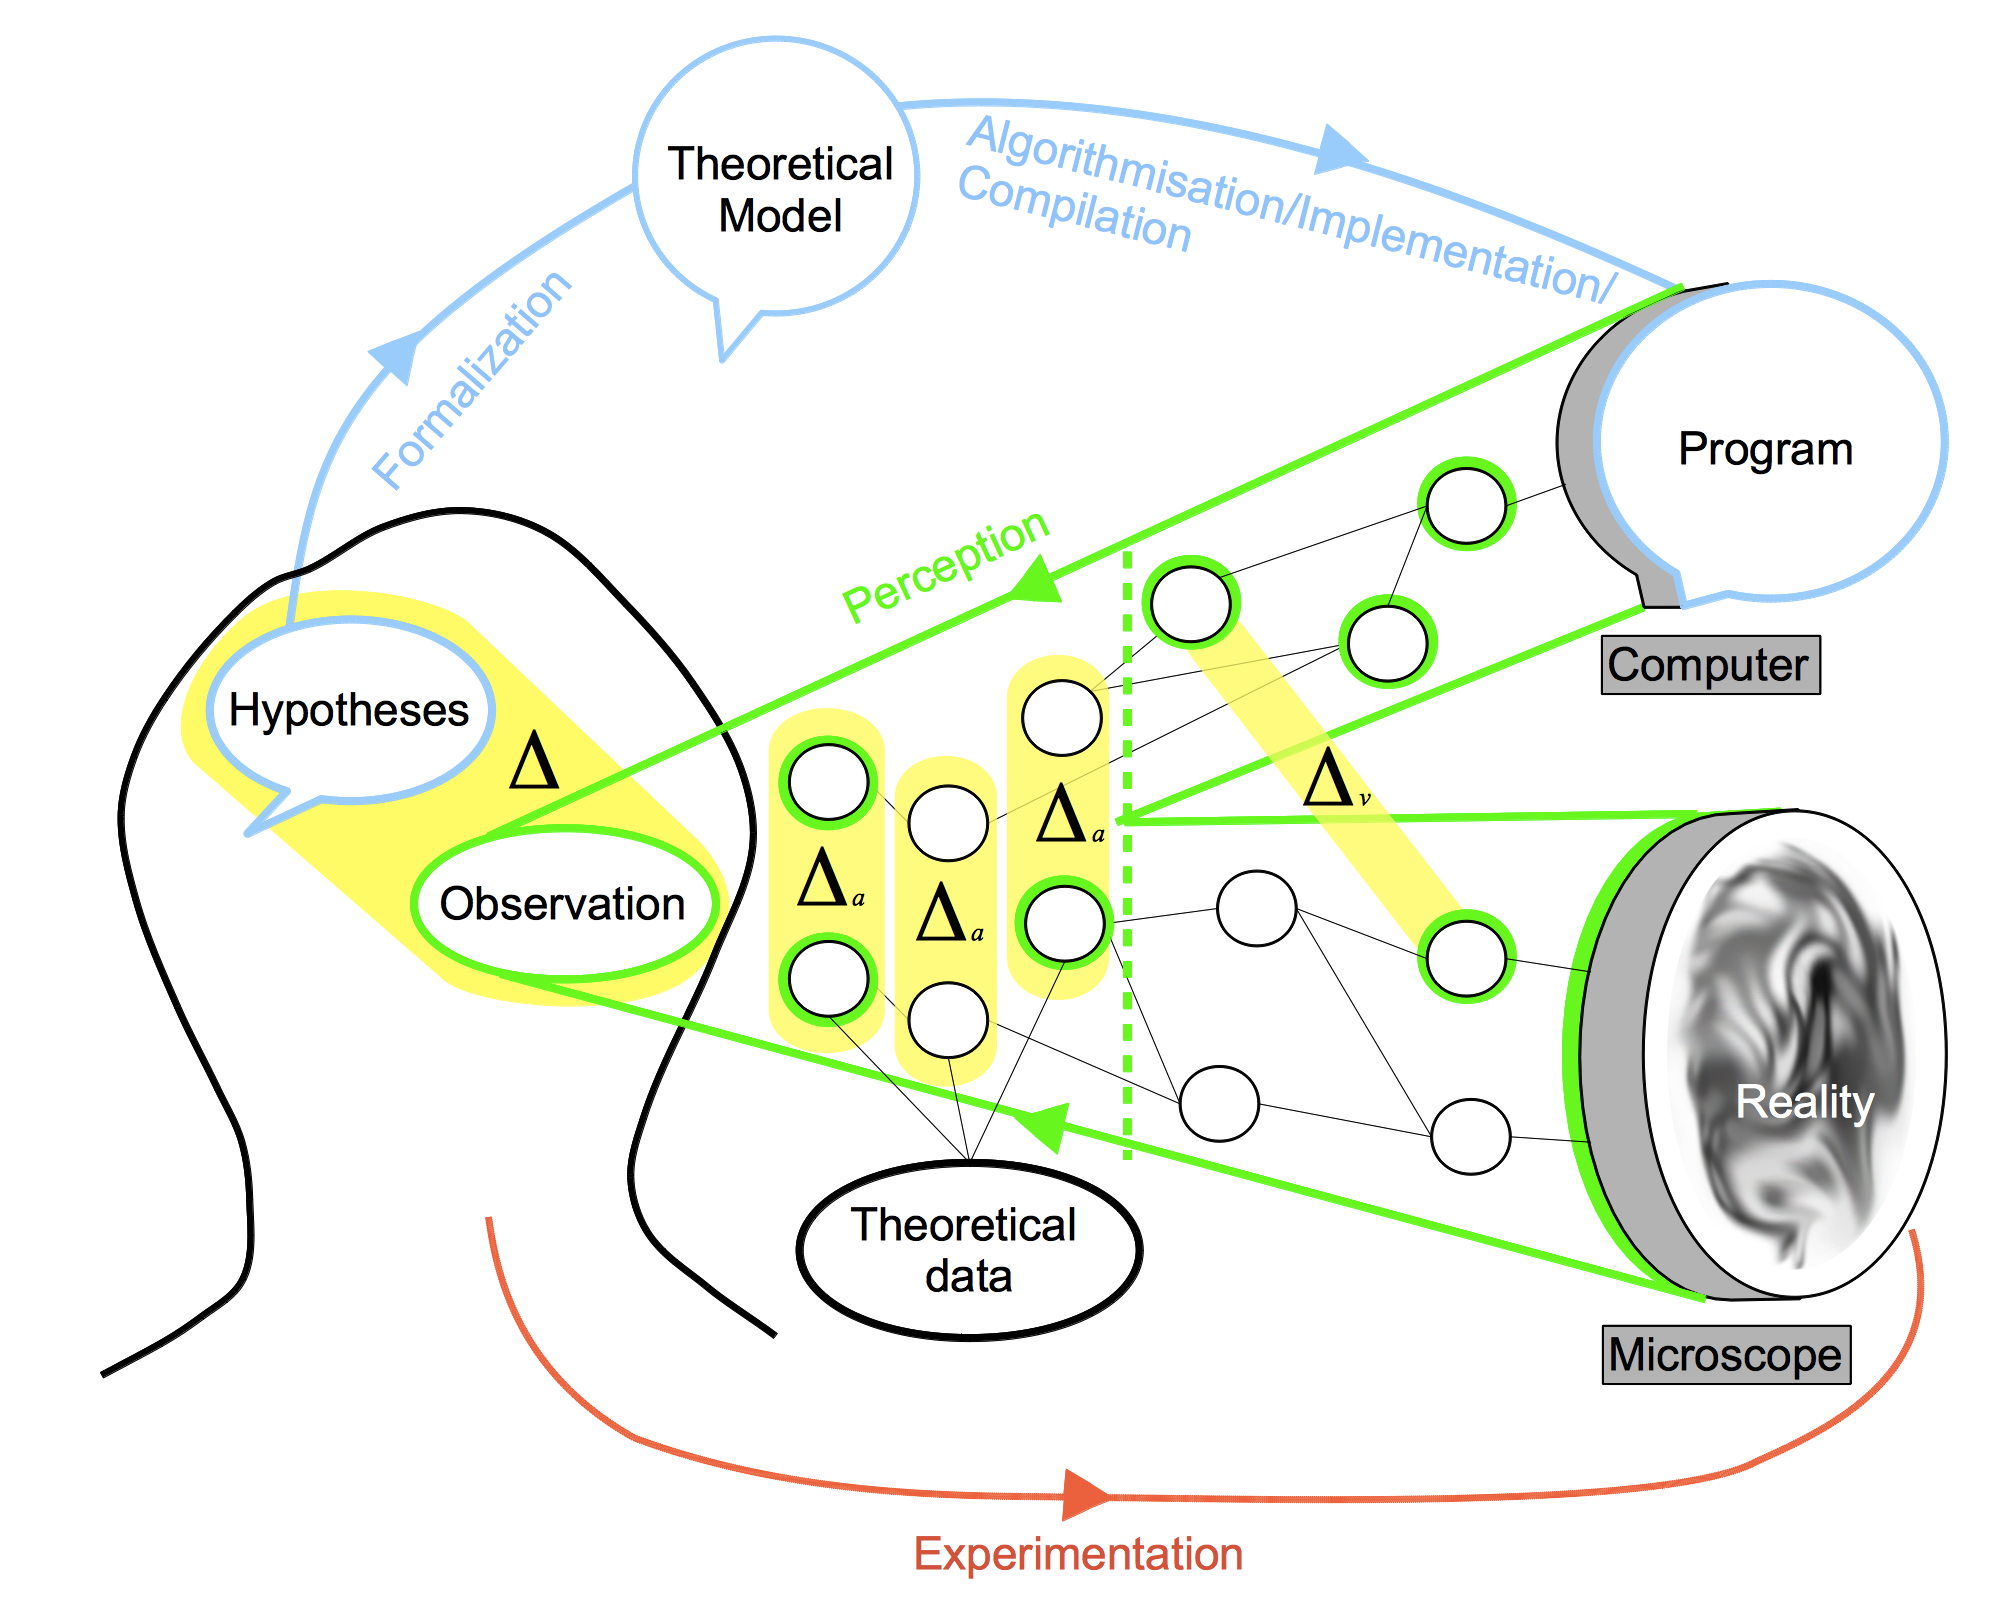
\includegraphics[width=0.6\textwidth]{../../images/experimental_science/experimental_science_larger_augmented.png}
\end{center}
\caption{\textbf{Integrative schematic of the tool-augmented observation-hypothesis-experiment loop.}}
\label{experimental_science_larger_augmented}
\end{figure}

\paragraph{Fitness function}
%  ++++++++++++++++++++++++++++++++++++++++++++++++++++++++++++++++++++++ 


The comparison between simulated and observed values is based on a "distance" between dynamical trajectories, which can be embodied by a \textit{fitness function} and applied to any one of the three categories of measures presented above (local, extensive or global). We distinguish between two types of fitness functions, in addition to the original "cognitive" comparison represented by the symbol $\Delta$ in Fig. \ref{experimental_science_larger_augmented}:
\begin{itemize}
	\item An \textit{automated fitness function}, denoted by $\Delta_a$: this function requires a reconstruction strategy based on the data generated by the simulation platform, similar to the reconstruction workflow described in the augmented perception part. It produces a quantitative score evaluating the discrepancy between two trajectories.
	\item A \textit{visual fitness function}, denoted by $\Delta_v$: the goal of this function is to support the individual's intuitions and hypotheses based on visualization only. Visual fitness is not as formalized as automated fitness, but it constitutes an important stepping stone toward automation (a continuation of the perception-augmenting tools) and was extensively used in this project.
\end{itemize}

\paragraph{Validation Schemes}
%  ++++++++++++++++++++++++++++++++++++++++++++++++++++++++++++++++++++++ 


There are at least two different scenarios of exploitation of this integrated platform, as the design of the model and its comparison with the observations are tightly coupled:
\begin{itemize}
	\item asserting the likelihood of the model by showing that the foundational hypotheses of the model are sufficient to mimic the observations in a satisfying manner
	\item conversely, assuming the validity of the model and optimizing its parameters, then using its predictive abilities to design new experiments.
\end{itemize}
\begin{figure}
\begin{center}
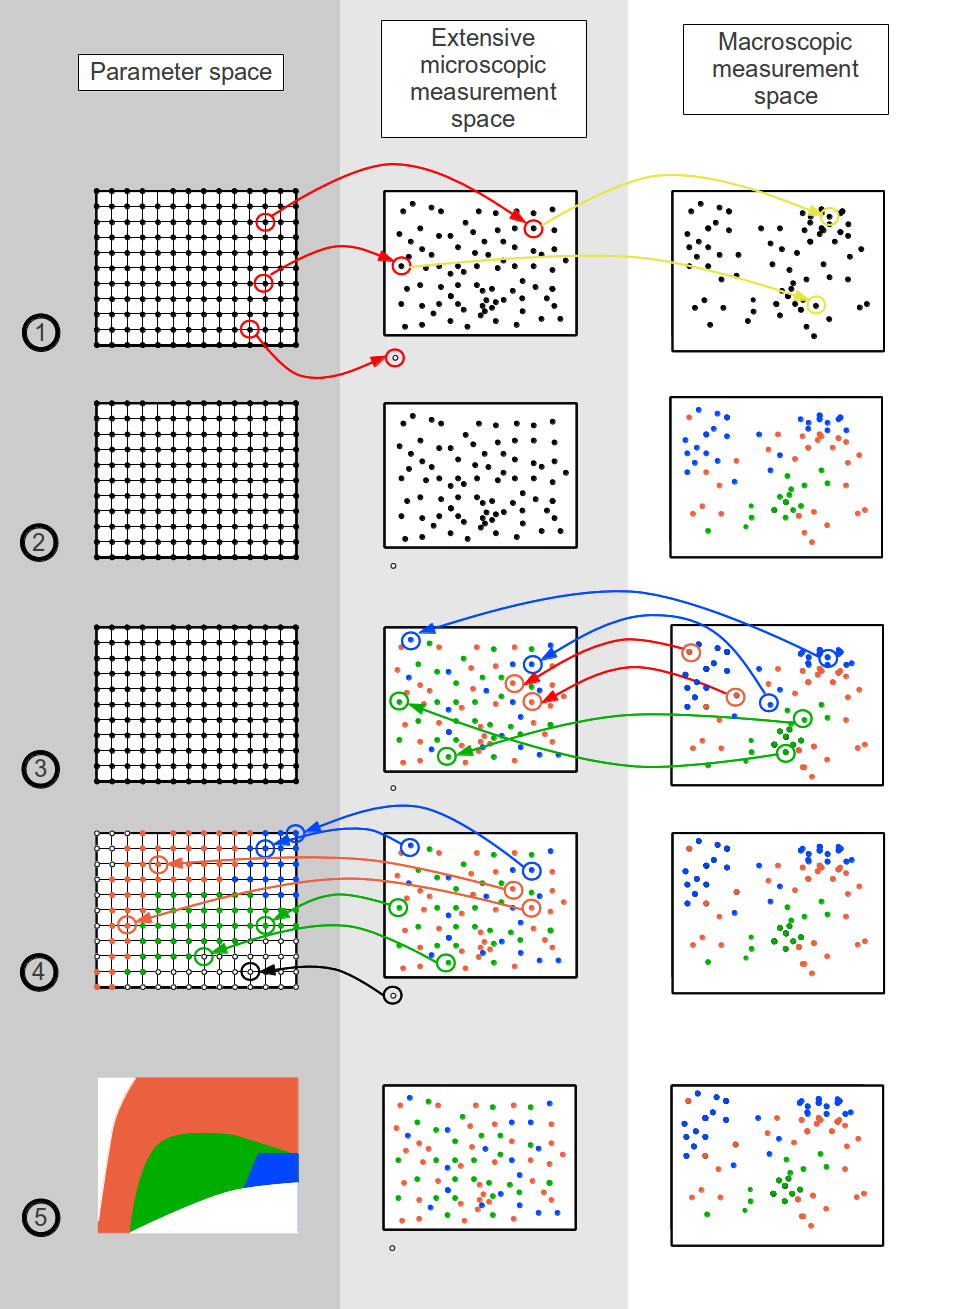
\includegraphics[width=0.8\textwidth]{../../images/experimental_science/phase_diagram2.png}
\end{center}
\caption{\textbf{ Generic evaluation of the performance of a model through quantitative evaluation of its parameter space.} To each element of the parameter space (left column), a deterministic dynamical system model associates a trajectory that may be represented by a single point in the extensive microscopic measurement space (this is the state space but we want to emphasize the complexity and the high dimensionality of this space when the model is agent-based, center column). The macroscopic measurement point are obtained by reconstructing and measuring the observations of interest in the complex trajectory space. Row 1 illustrates the passage from the parameter space to the extensive microscopic measurement space (red arrows). As shown by the arrow pointing to the white dot, there is no guaranty that every point in the parameter space produces a "viable" trajectory. Quantitative assessment of the performance of the trajectory are determined according to adapted criteria (comparison with a target measure Fig. \ref{experimental_science_phase_diagram_distance}, clustering). A "color" is attributed to the macroscopic measure points to symbolize this evaluation (Row 2). The color is easily propagated back to the parameter space and allows a quantitative assessment of the performance of every trajectory (Row 3, 4, 5). White regions represent parts of the parameter space that are not viable (Row 5).}
\label{experimental_science_phase_diagram2}
\end{figure}

This scheme can be easily generalized to compare (Fig. \ref{experimental_science_phase_diagram_distance}):
\begin{itemize}
	\item two or more models
	\item two or more individuals within a cohort (population of experimental individuals with the same a priori initial state, including genetic and environmental conditions)
	\item individuals from different cohorts
	\item models and theoretical data plotted in the macroscopic measure space.
\end{itemize}
\begin{figure}
\begin{center}
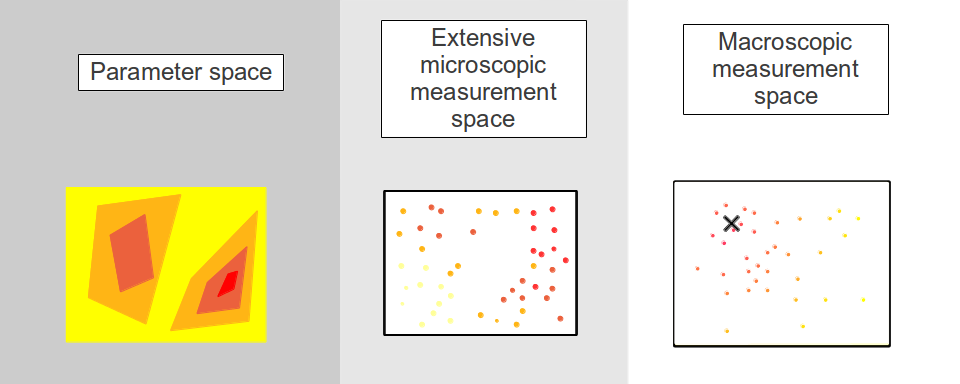
\includegraphics[width=0.8\textwidth]{../../images/experimental_science/phase_diagram_distance.png}
\end{center}
\caption{\textbf{Fitness landscape according to a target macroscopic measure.} This schema is a particular example illustrating the case of a model evaluated by the comparison a macroscopic measure (black cross). The score of each trajectory is attributed as a function of the distance between the simulated macroscopic measures and the target macroscopic measure.}
\label{experimental_science_phase_diagram_distance}
\end{figure}

An orthogonal distinction among fitness functions focuses on the type of observed data and simulated data that are compared (Fig. \ref{experimental_science_experimental_science_cleaner}):
\begin{itemize}
	\item Reconstruction of experimental raw data: we call this fitness function \textit{experimental reconstruction fitness} (ERF).
	\item Theoretical data representing an idealized phenotypic behavior: we call this fitness function \textit{theoretical fitness} (TF).
\end{itemize}
\begin{figure}
\begin{center}
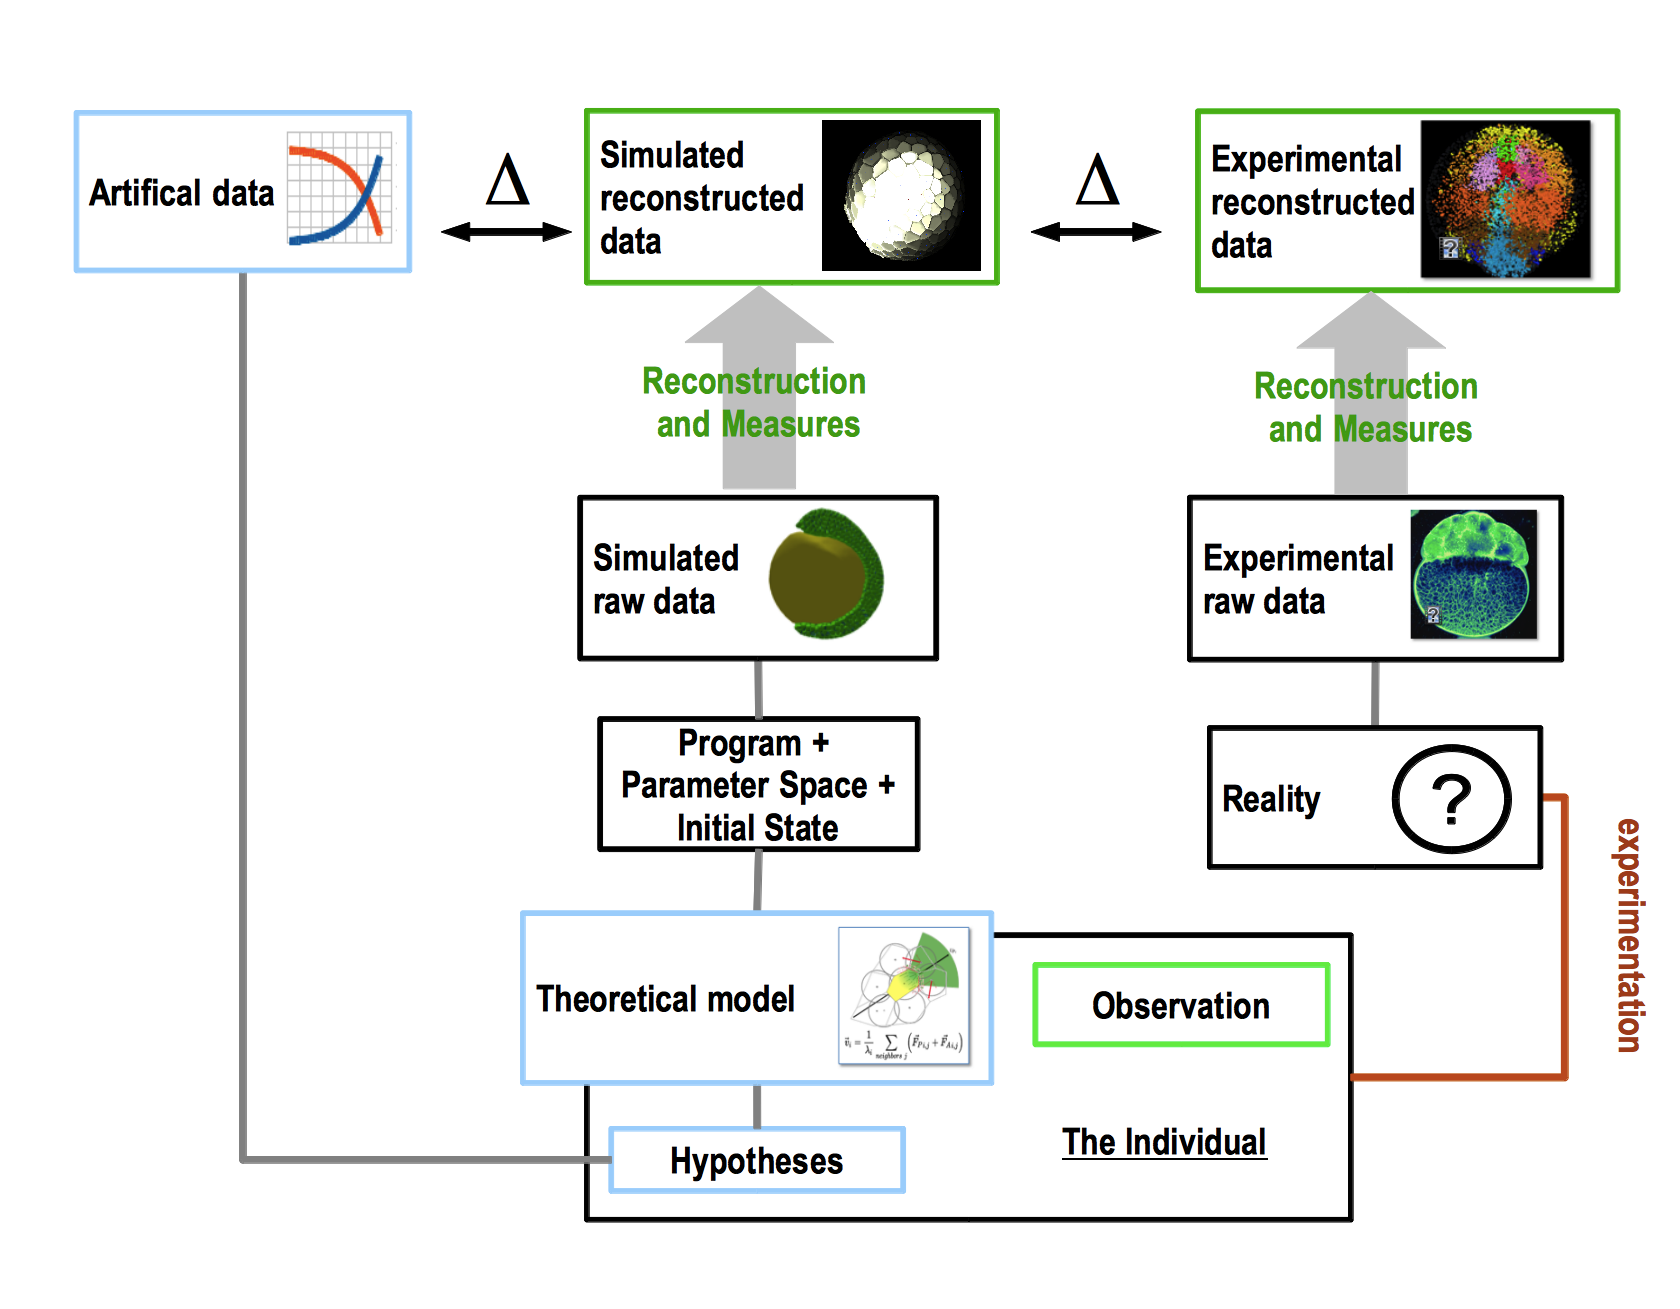
\includegraphics[width=0.95\textwidth]{../../images/experimental_science/experimental_science_cleaner.png}
\end{center}
\caption{\textbf{Summary of the methodological workflow adopted for this project.} The top left $\Delta$ symbolizes the theoretical fitness (TF) and the top right $\Delta$ the experimental reconstruction fitness (ERF).}
\label{experimental_science_experimental_science_cleaner}
\end{figure}
%  ====================================================================== 


\subsection{Overview of this Dissertation}
%  ====================================================================== 
  ...  Expliquer le stratégie qui consiste à commencer par la mécanique avant la génétique voir argument de Murray (p.314 \cite{Murray:2003ty}):  "However one chooses to ignore mechanics, nevertheless, presiding over every embryonic twitch and jerk are Newton’s laws. And whatever role chemistry and genetics play in embryogenesis, they must finally submit their programs for Newtonian execution. Therefore, we have adopted the philosophy that, since morphogenesis is—at least proximally—a mechanical event, it is reasonable to start analyses of morphogenetic processes by examining the forces that produced them, and then, working backwards, add chemistry and genetics as needed."  ...   Discussion globale, en attendant de créer un chapitre  nouveau type de microscopie  -> electronique, voir CLEM, on freeze l'embryon, on le découpe, on peut voir les structures subcellulaire, membranes et surtout marquer les anticorps donc imager n'importe quoi  
